% Chapter 1

\chapter{Application Implementation} % Write in your own chapter title
\label{Application Implementationn}
\lhead{Chapter 5. \emph{Application Implementation}} % Write in your own chapter title to set the page header

\section{introduction}

In chapter 3 we summarized the sequence of actions that occurred during the application's design part. In this chapter we will go through the implementation phase, outlining the core functionalities of the application. In addition, screen shots illustrating the application in action will be provided. Furthermore, a description about how the application was tested will be presented, along with the appropriate unit tests that were run. The chapter ends with a discussion and criticism about the final outcome of the implementation phase along with future work.

\section{Application's Implementation Phase}

In this section we will present how the application was implemented based on the decisions that were taken during the design phase. More specifically, we will introduce a set of sequence diagrams, illustrating the flow of function calls. The diagrams will be accompanied by a brief description, as well as, several screenshots showing the application in action.

\subsection{Add Trip}

As explained earlier, this use case requires users to insert the trips that they make during the course of time. The sequence diagram in figure \ref{fig:addTripInfoSeqDiagram} illustrates the process of adding information about the trips, whereas the sequence diagram in figure \ref{fig:tripStoreSeqDiagram} demonstrates the flow of function calls that take place so that the information users insert is stored in a persistent database.

Figure \ref{fig:addTripForm} illustrates a web user interface for the trip creation process. The red rectangle indicates the \emph{addTripview} Ember view which is the main form for adding new trips. The tripLegContainer is shadowed with the blue rectangle and is, essentially, an Ember container view\footnote{$http://docs.emberjs.com/doc=Ember.ContainerView$} capable of dynamically adding new sub-views, such as \emph{tripLegView} for each trip. Finally, the yellow rectangle shows the carView view.

The sequence diagram \ref{fig:addTripInfoSeqDiagram} shows a scenario where the user initially inserts information concerning the trip's name, type, date and number of trip legs. When choosing the number of trip legs, the \emph{tripLegContainer} is created which in turn creates a number of \emph{tripLegView} views based on the number of trip legs. Then user again needs to indicate some information about the trip leg's source and destination address, and the transport mean that was used. Selecting a transport mean, results in the creation of the \emph{tripLegTransportContainer} view, which is a dynamic view that we have used to support rich interactivity. In this scenario, user has chosen a car; therefore a \emph{carView} view (yellow rectangle) is added to the \emph{tripLegTransportContainer}. The form element in that view are populated with data that are fetched from the back-end via AJAX GET calls. Finally, after filling all the required fields, the user submits the form.

\begin{landscape}
\begin{figure}[htbp]
	\centering
		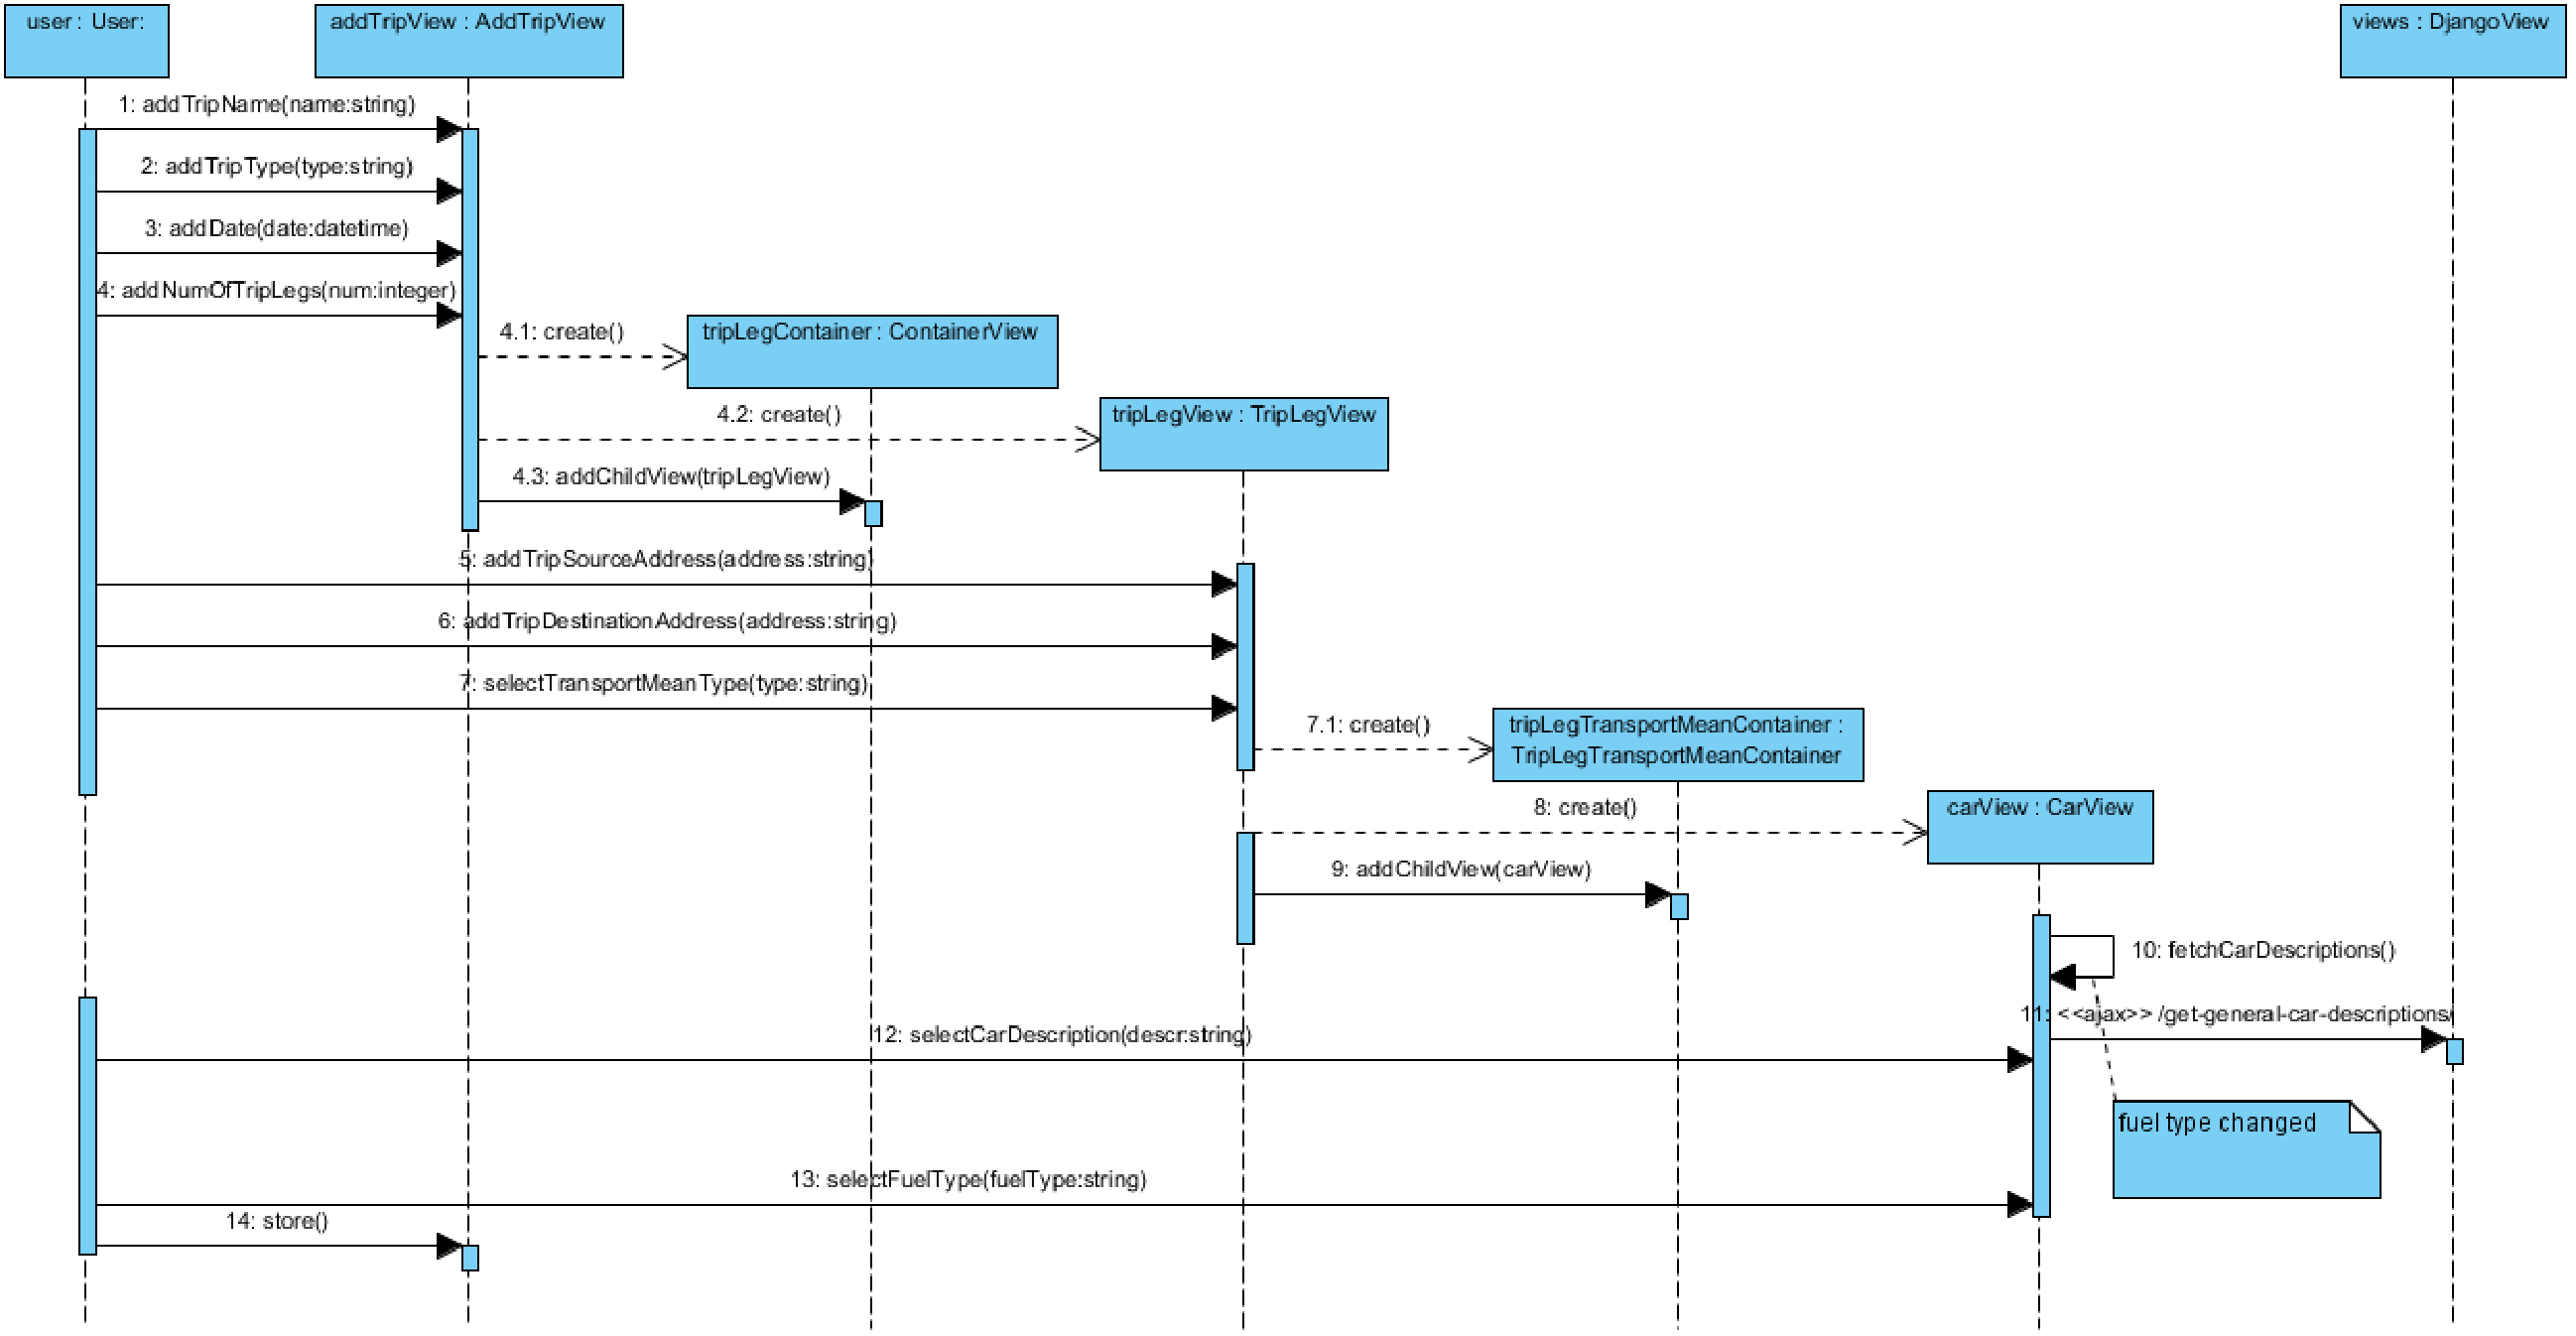
\includegraphics[scale=0.55]{./Figures/chapter4/figure10.pdf}
		\rule{35em}{0.5pt}
	\caption[Add trip information sequence diagram]{Add trip information sequence diagram}
	\label{fig:addTripInfoSeqDiagram}
\end{figure}
\end{landscape}

\begin{figure}[htbp]
	\centering
		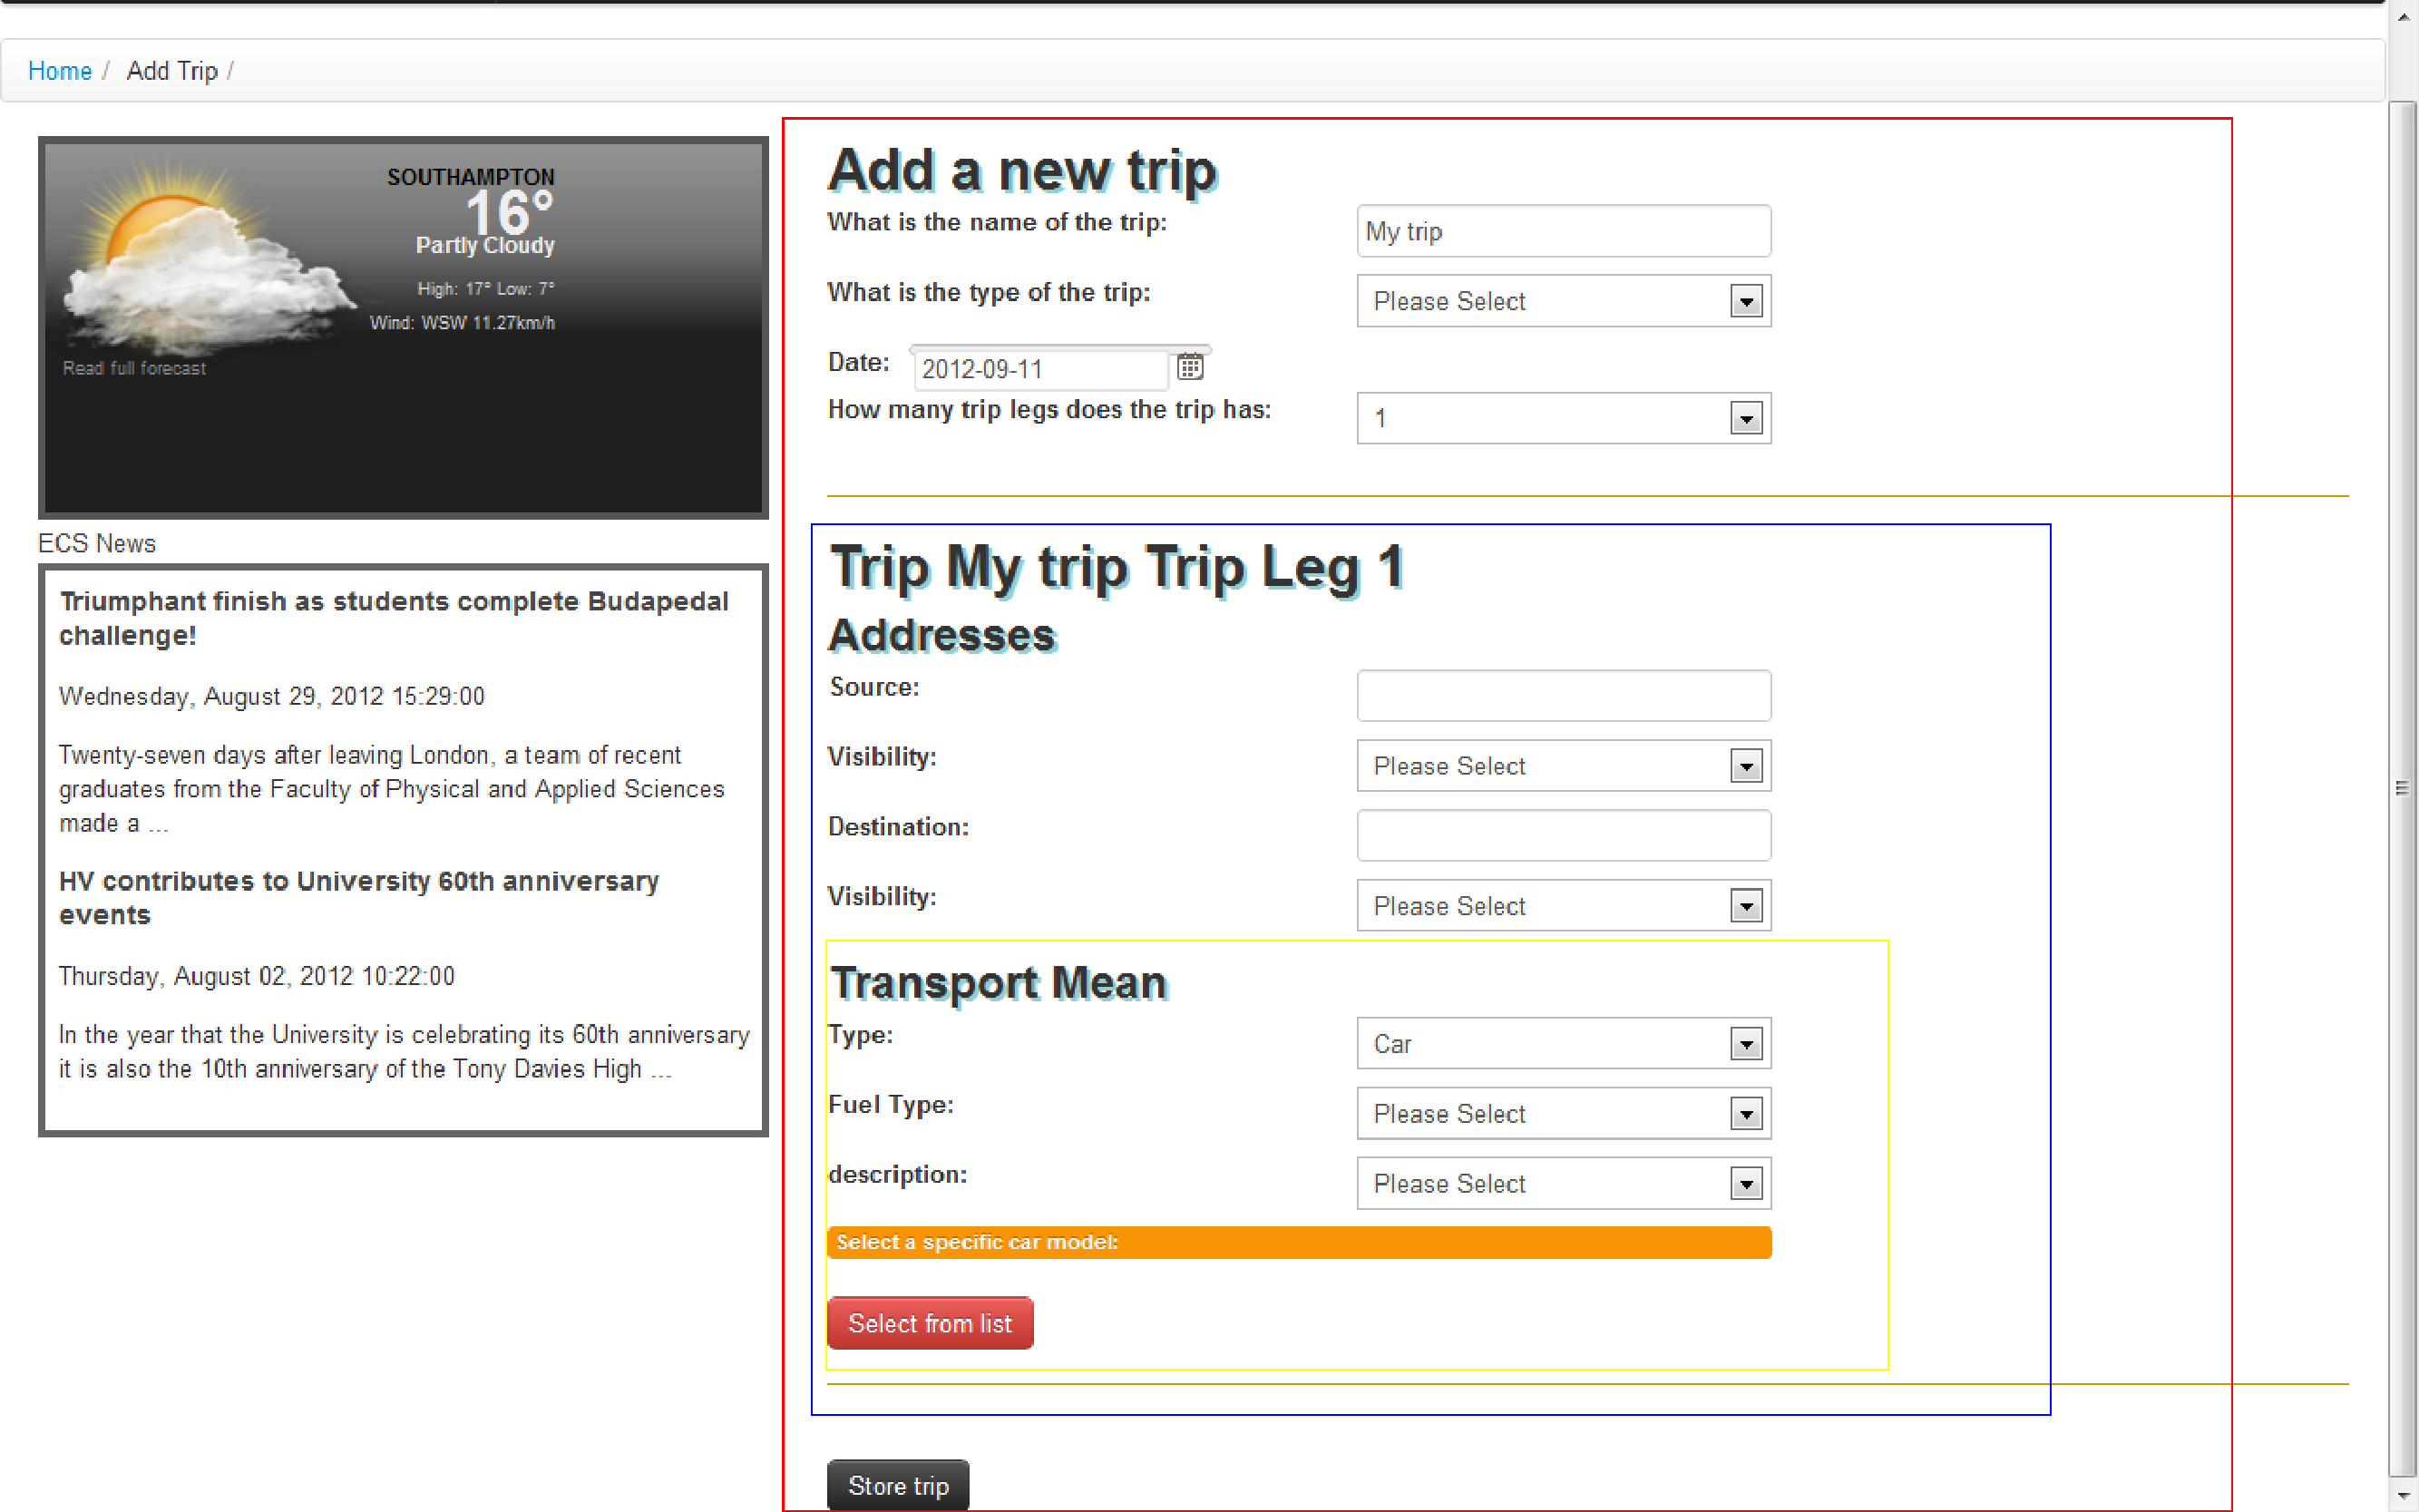
\includegraphics[scale=0.40]{./Figures/chapter4/figure12.pdf}
		\rule{35em}{0.5pt}
	\caption[Add trip from]{Add trip form}
	\label{fig:addTripForm}
\end{figure}

The process of storing a trip starts after the user submits the trip creation form, that we described earlier. Initially, the \emph{tripManagerController} compiles the data inserted by the user and fills the corresponding models, namely tripLegModel and generalCarModel. It then makes an AJAX Post call to the back end, sending information about the trip. On the back-end, the corresponding view creates a trip model and stores it in the database. On the next step, the controller makes consequent AJAX Post request, asking for the back end to store each trip leg into the database. Finally, two more AJAX calls occur; the first asks the back-end to create a provenance graph for each trip leg, whereas the second asks for the carbon emissions of each trip leg to be calculated.

\begin{landscape}
\begin{figure}[htbp]
	\centering
		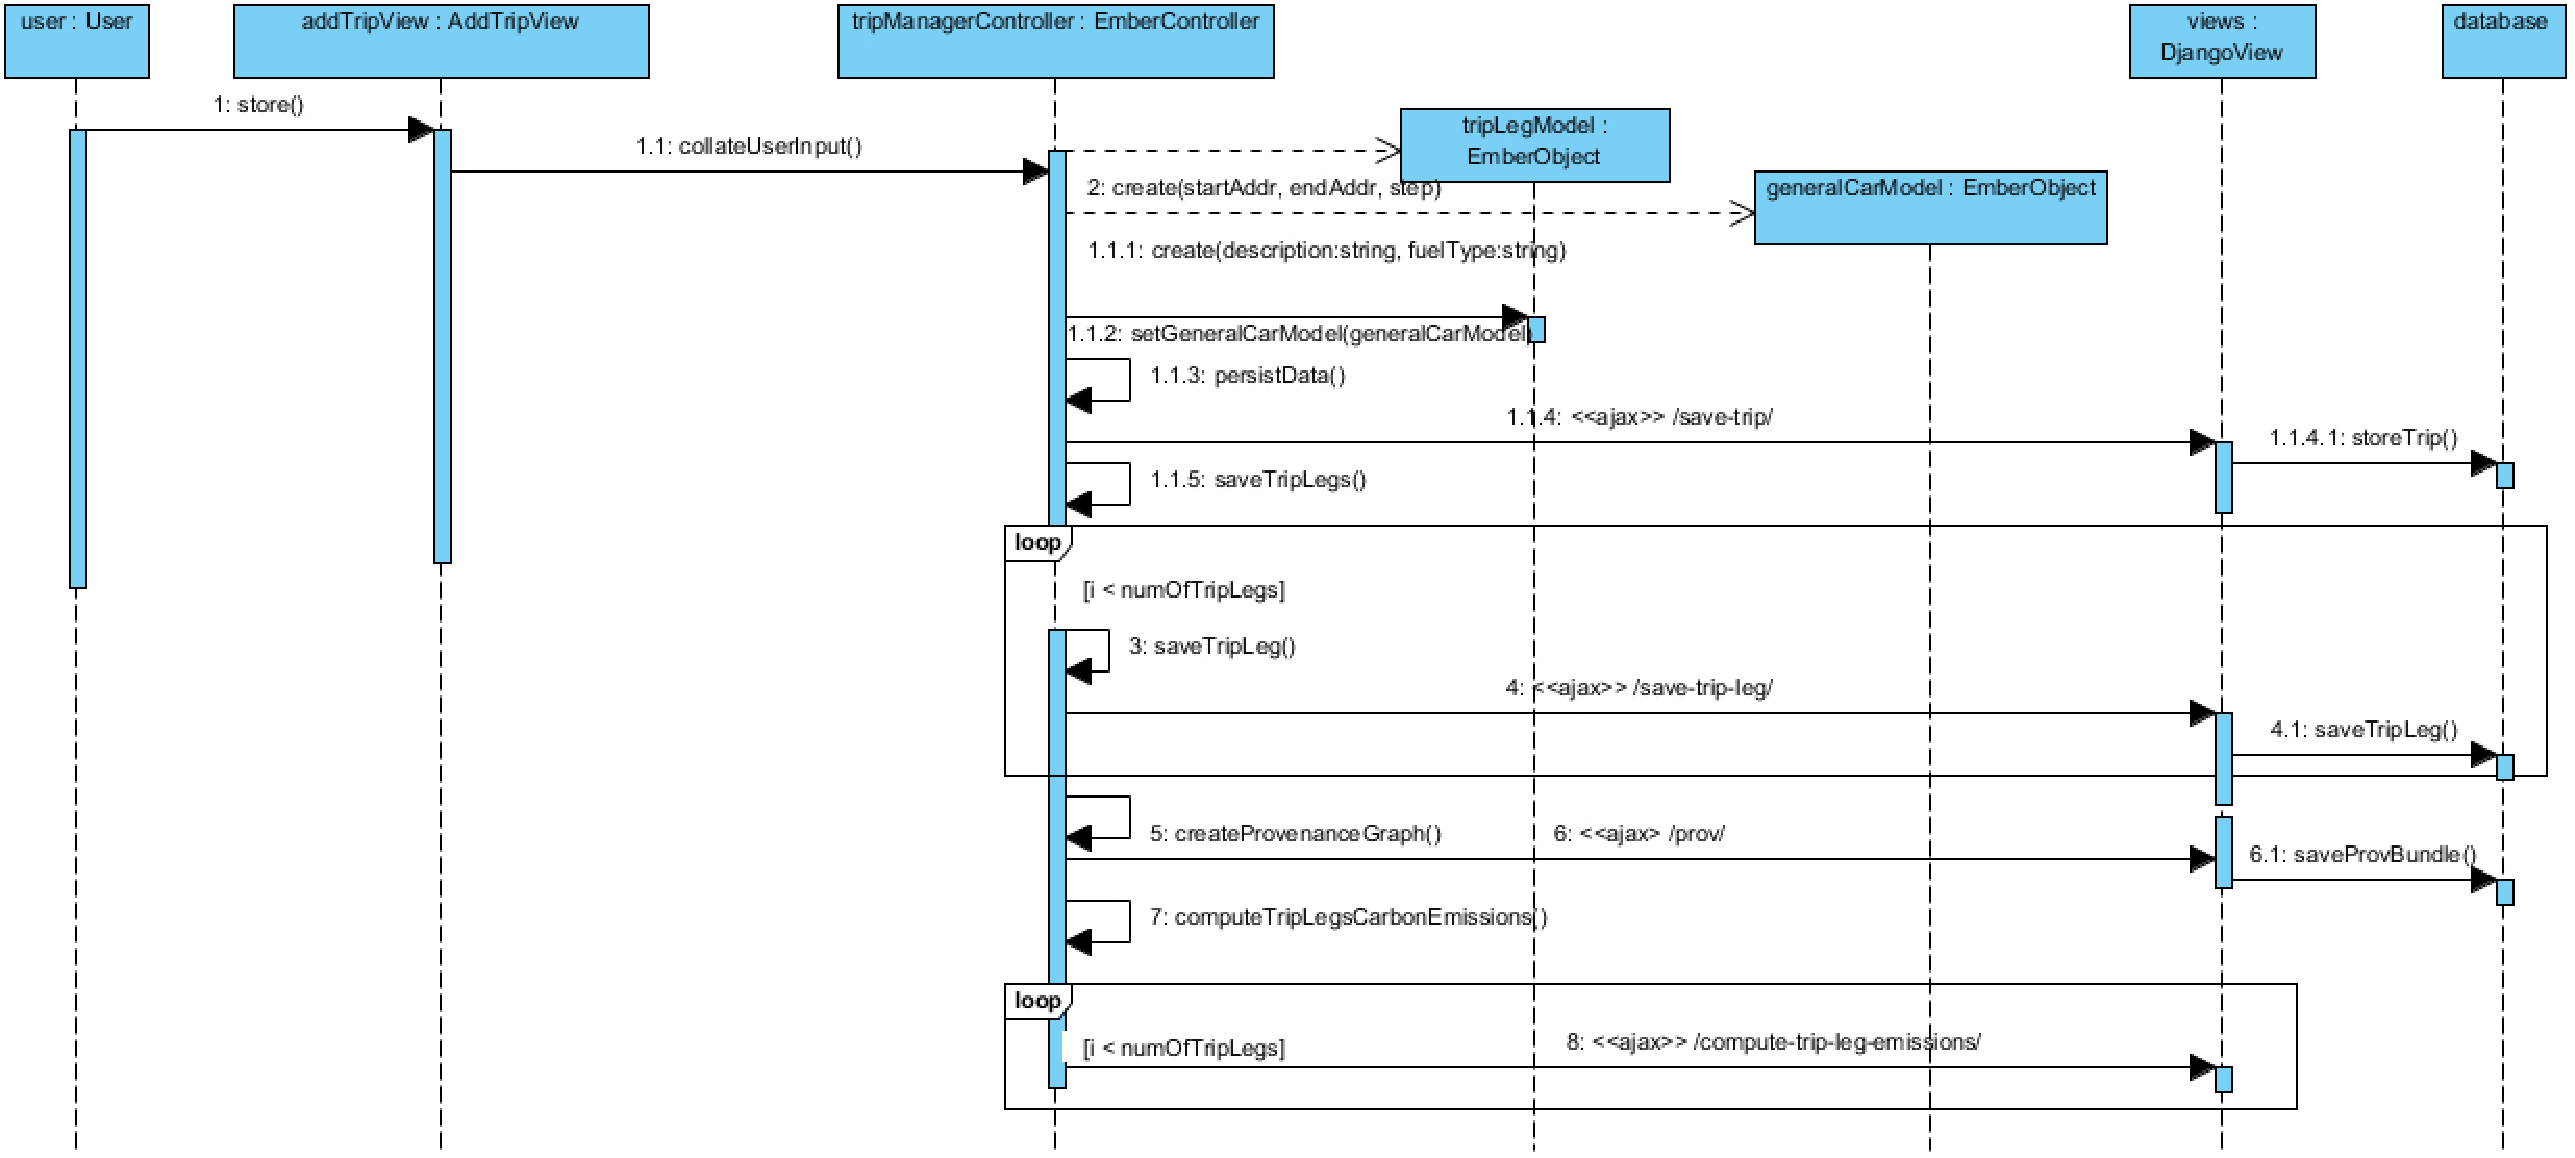
\includegraphics[scale=0.55]{./Figures/chapter4/figure13.pdf}
		\rule{35em}{0.5pt}
	\caption[Trip storing sequence diagram]{Trip storing sequence diagram}
	\label{fig:tripStoreSeqDiagram}
\end{figure}
\end{landscape}

\subsection{Show User's Trips}

The user have the chance to manage the trip that he has added to the system. More specifically, the actions that are offered are: view, edit and delete tips. Figure \ref{fig:userTrips} illustrates the web user interface that displays all user's trips. Notice that trips are categorized according to the transport means that were used.

\begin{figure}[htbp]
	\centering
		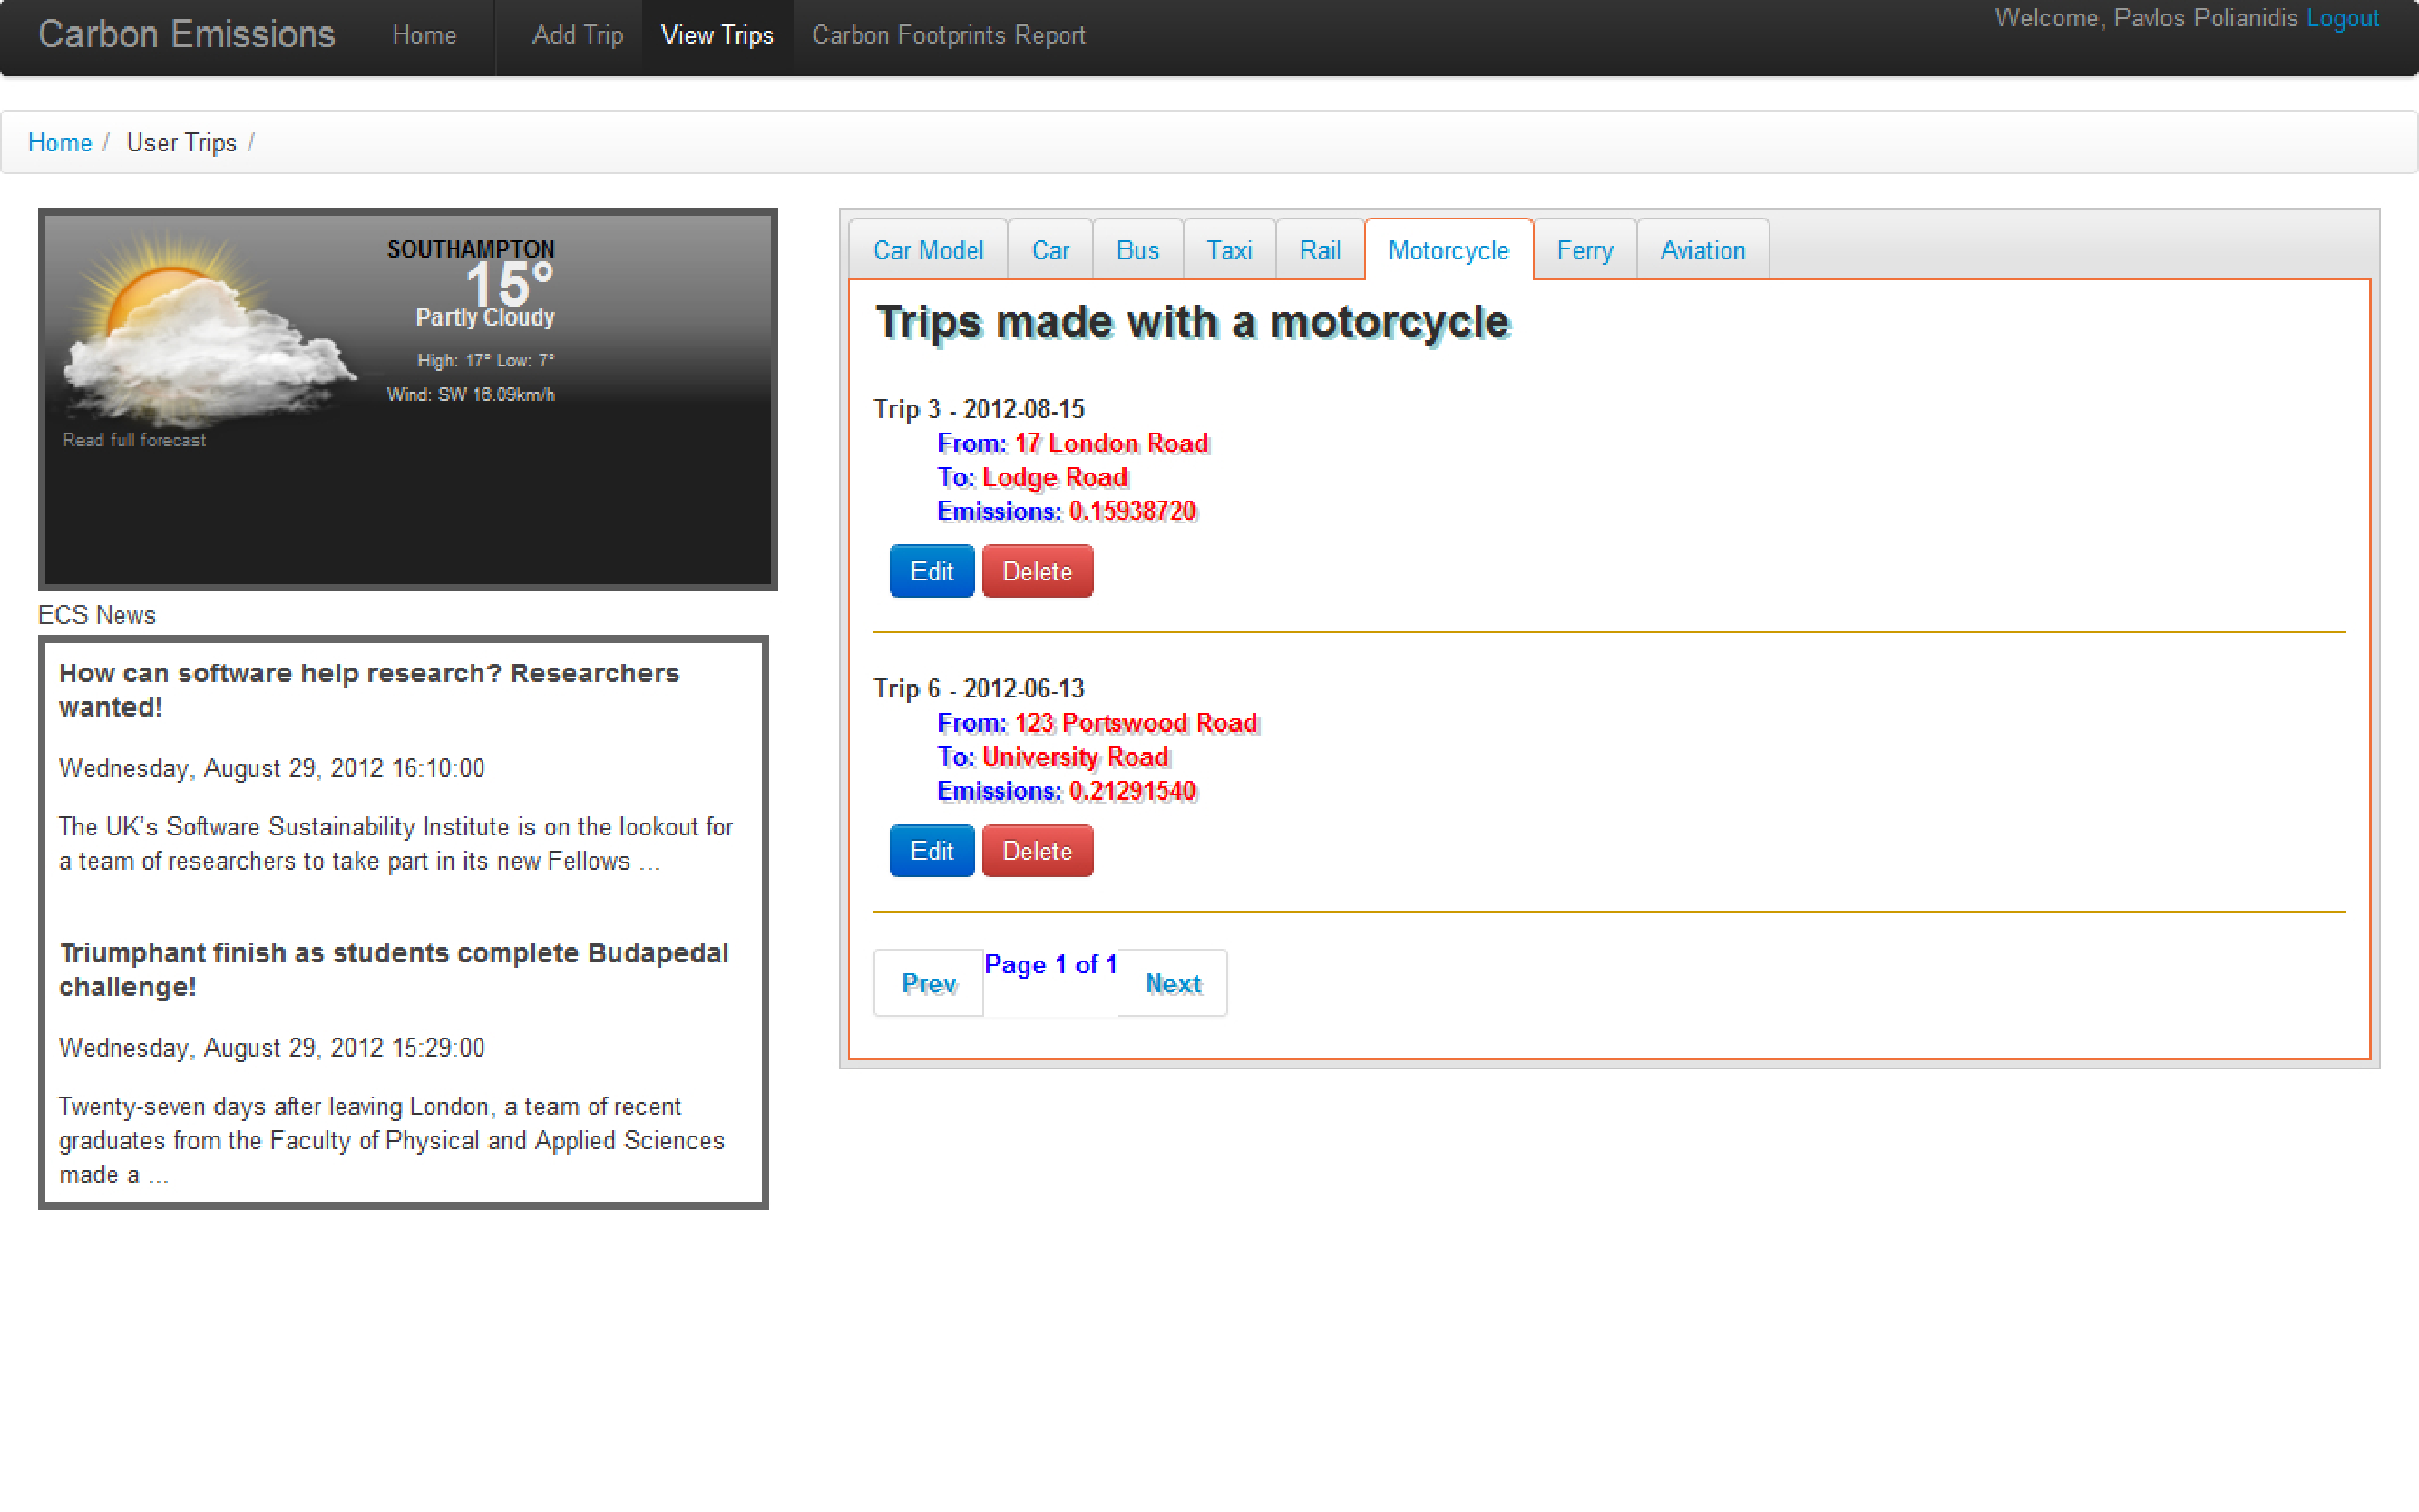
\includegraphics[scale=0.40]{./Figures/chapter4/figure14.pdf}
		\rule{35em}{0.5pt}
	\caption[UI showing user's trips]{UI showing user's trips}
	\label{fig:userTrips}
\end{figure}

As shown in the sequence diagram \ref{fig:userTripsSeqDiagram} the process is fairly simple. The \emph{tripInfoController} fetches the trips made by a car from the back-end via an AJAX GET request. The back-end, in order, retrieves those data from the database and returns the in JSON format.

\begin{landscape}
\begin{figure}[htbp]
	\centering
		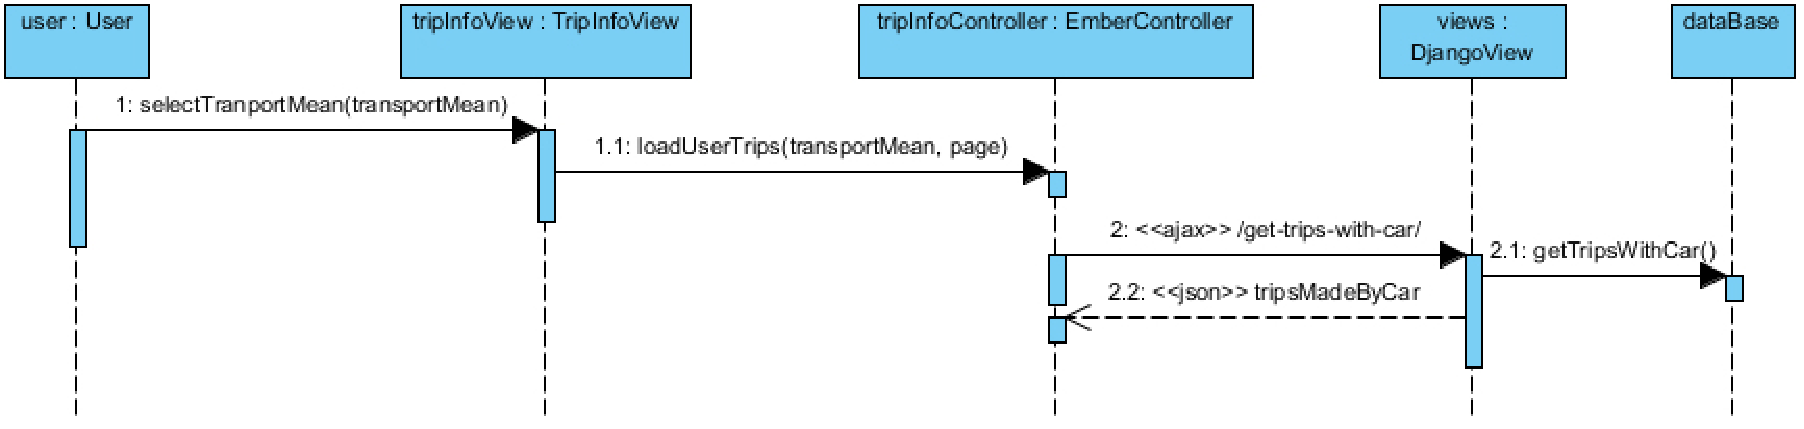
\includegraphics[scale=0.55]{./Figures/chapter4/figure15.pdf}
		\rule{35em}{0.5pt}
	\caption[Displaying user's trips sequence diagram]{Displaying user's trips sequence diagram}
	\label{fig:userTripsSeqDiagram}
\end{figure}
\end{landscape}

\subsection{Carbon Footprint Report}

The prime incentive for users adding the trips they make is to present a report describing their individual, as well as, group carbon footprints. In its current state, the application supports visualization of carbon emissions in the form of line and bar charts. Furthermore, the provenance for trip legs' carbon emissions are illustrated with two types of graphs; dynamic and static provenance graphs. We will expand on that in a bit. Figure \ref{fig:reportOverview} illustrates the a small part of report html page (/report).

\begin{figure}[htbp]
	\centering
		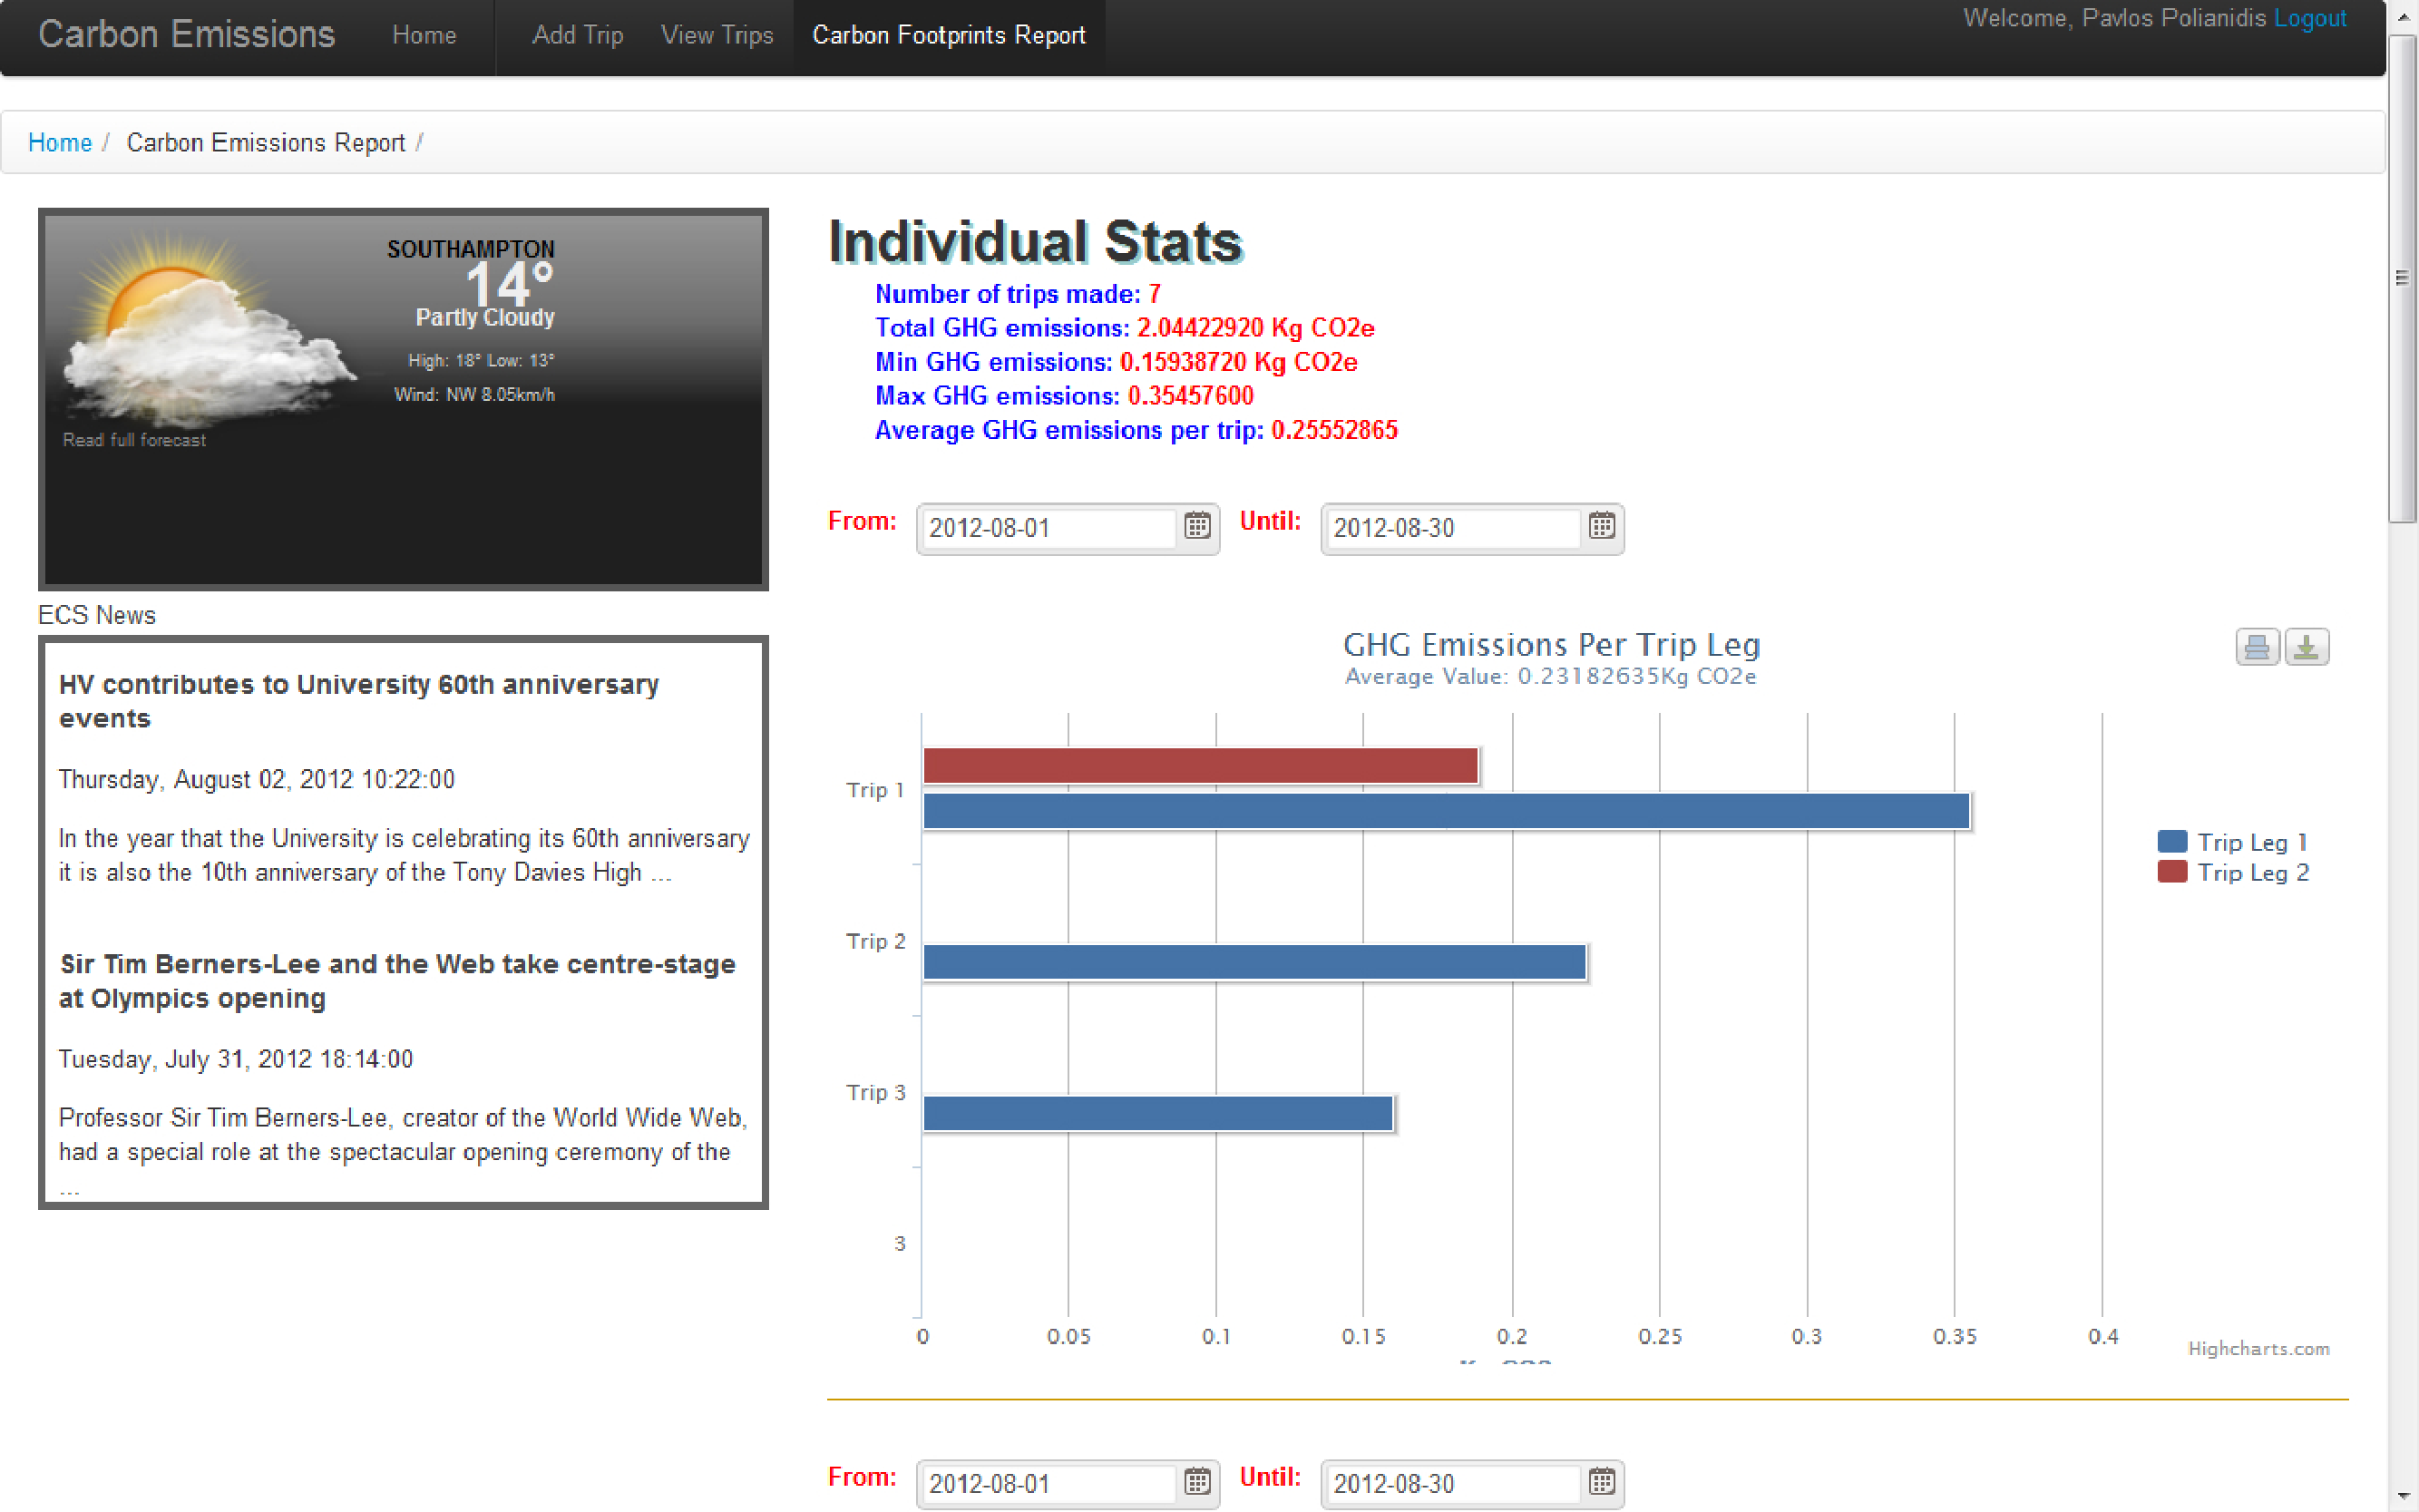
\includegraphics[scale=0.40]{./Figures/chapter4/figure16.pdf}
		\rule{35em}{0.5pt}
	\caption[Carbon footprint report page]{Carbon footprint report page}
	\label{fig:reportOverview}
\end{figure}


\subsubsection{Individual Carbon Emissions}

Users can view a small summary of their carbon footprints at the top of the report page. In its current state, the application presents the following statistics (view figure \ref{fig:ghgPerTripLeg}).

\begin{itemize}
  \item The number of trips that a user has made overall.
  \item The total weight of greenhouse gas emissions (ghg) caused by user's travels.
  \item The minimum value of greenhouse gas emissions.
  \item The maximum value of greenhouse gas emissions.
  \item The average weight of greenhouse gas emissions (ghg) caused by user's travels.
\end{itemize}

Apart from that, the report includes four charts presenting different information each. The first chart (figure \ref{fig:ghgPerTripLeg}) summarizes the carbon emissions caused by trip legs, during a specified period of time. By default, the application shows the emissions during the current month. Nevertheless, users can define the time period with the aid of two calendar widgets that reside on the top of each chart. Additionally, all the charts can be printed and downloaded in several formats, namely in PNG, PDF, JPEG and SVG.

\begin{figure}[htbp]
	\centering
		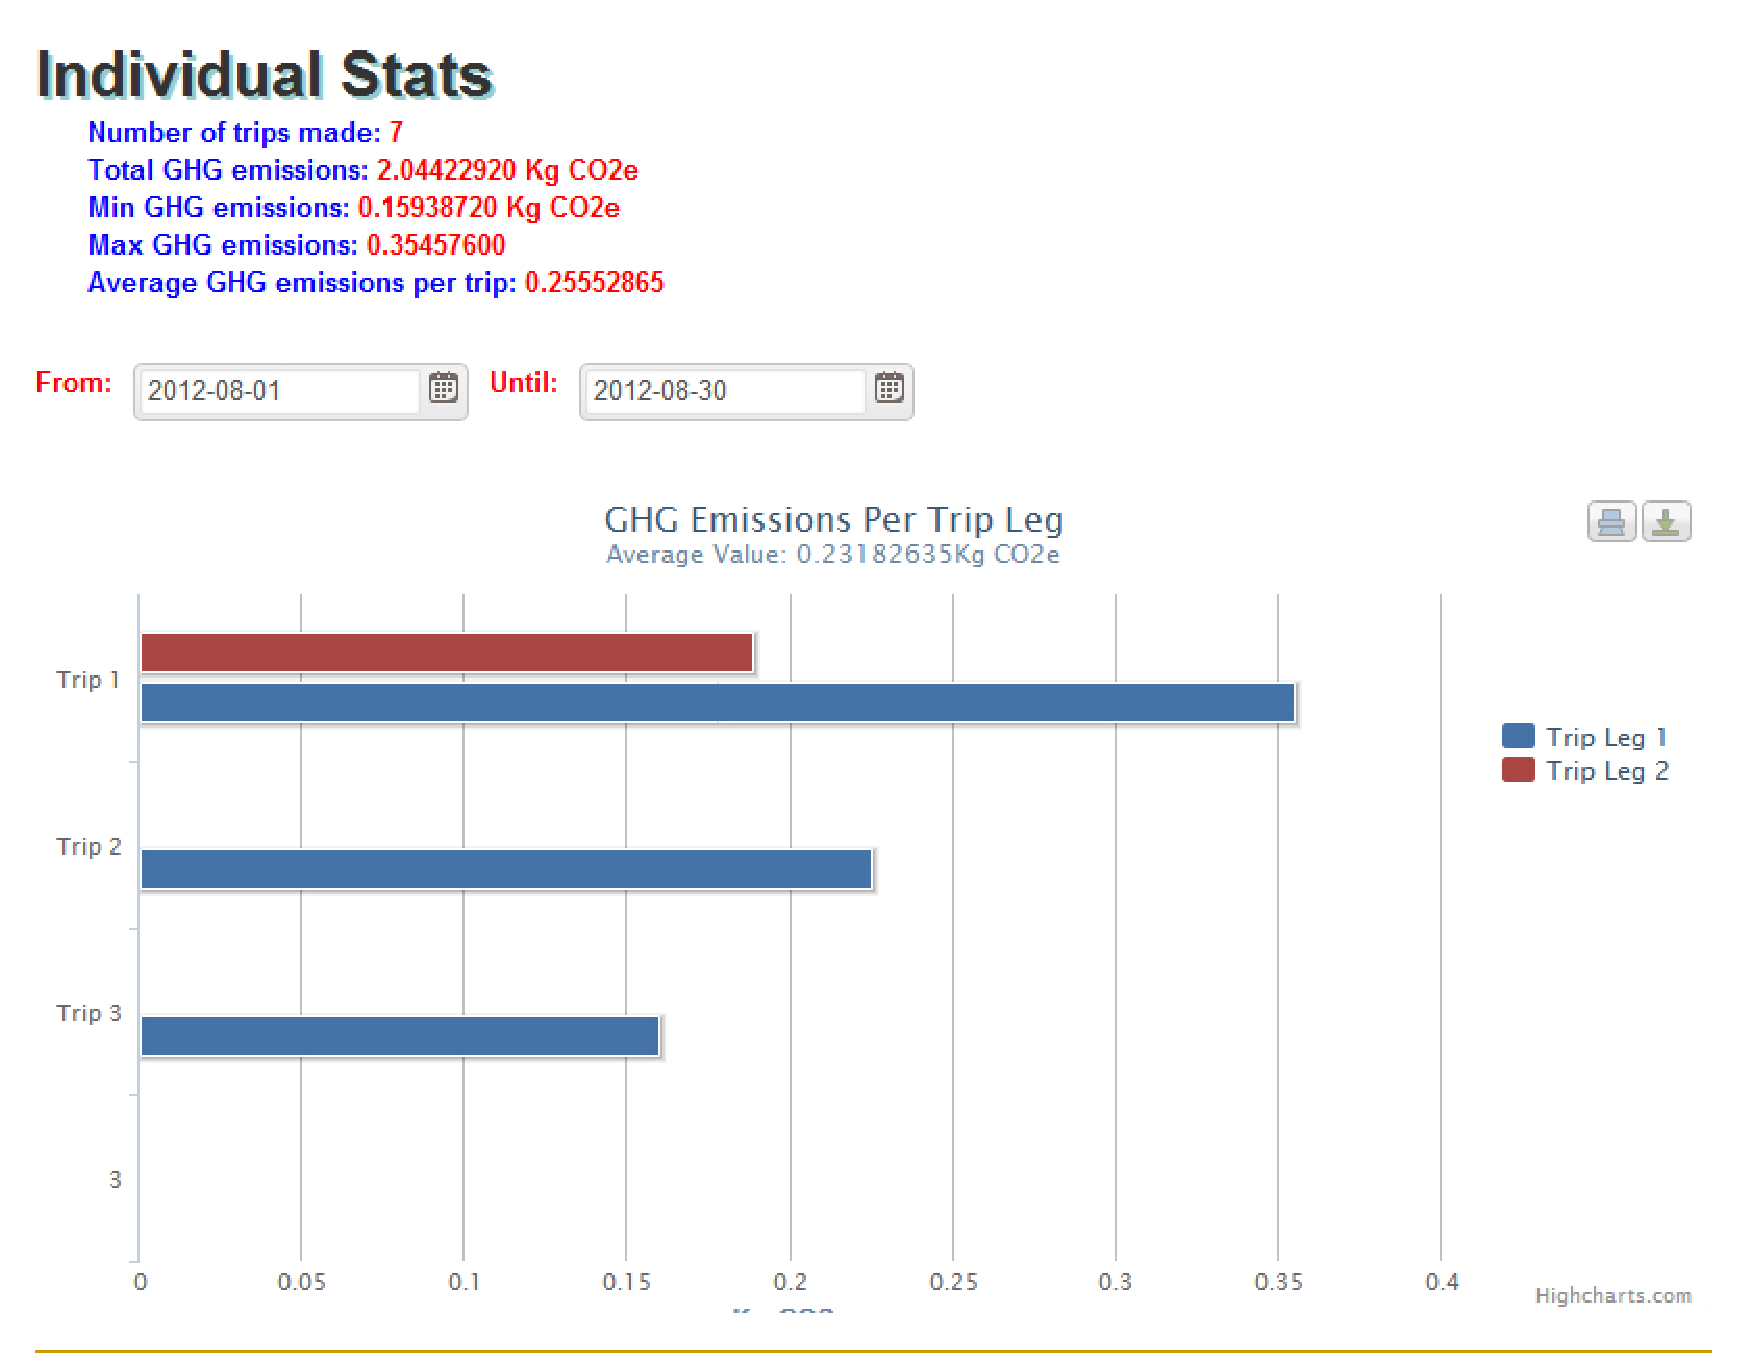
\includegraphics[scale=0.60]{./Figures/chapter4/figure17.pdf}
		\rule{35em}{0.5pt}
	\caption[Greenhouse gas emissions per trip leg]{Greenhouse gas emissions per trip leg}
	\label{fig:ghgPerTripLeg}
\end{figure}

As a complement to that chart, users can view the provenance graph of each trip leg carbon emission value. This is done by clicking on any bar; for instance, clicking on the first bar, the provenance information describing the derivation of that value, will appear (view figure \ref{fig:provGraph}). This is a interactive graph, in that, users can relocate the nodes, zoom in and zoom out, and click on each node to view a brief description.

\begin{figure}[htbp]
	\centering
		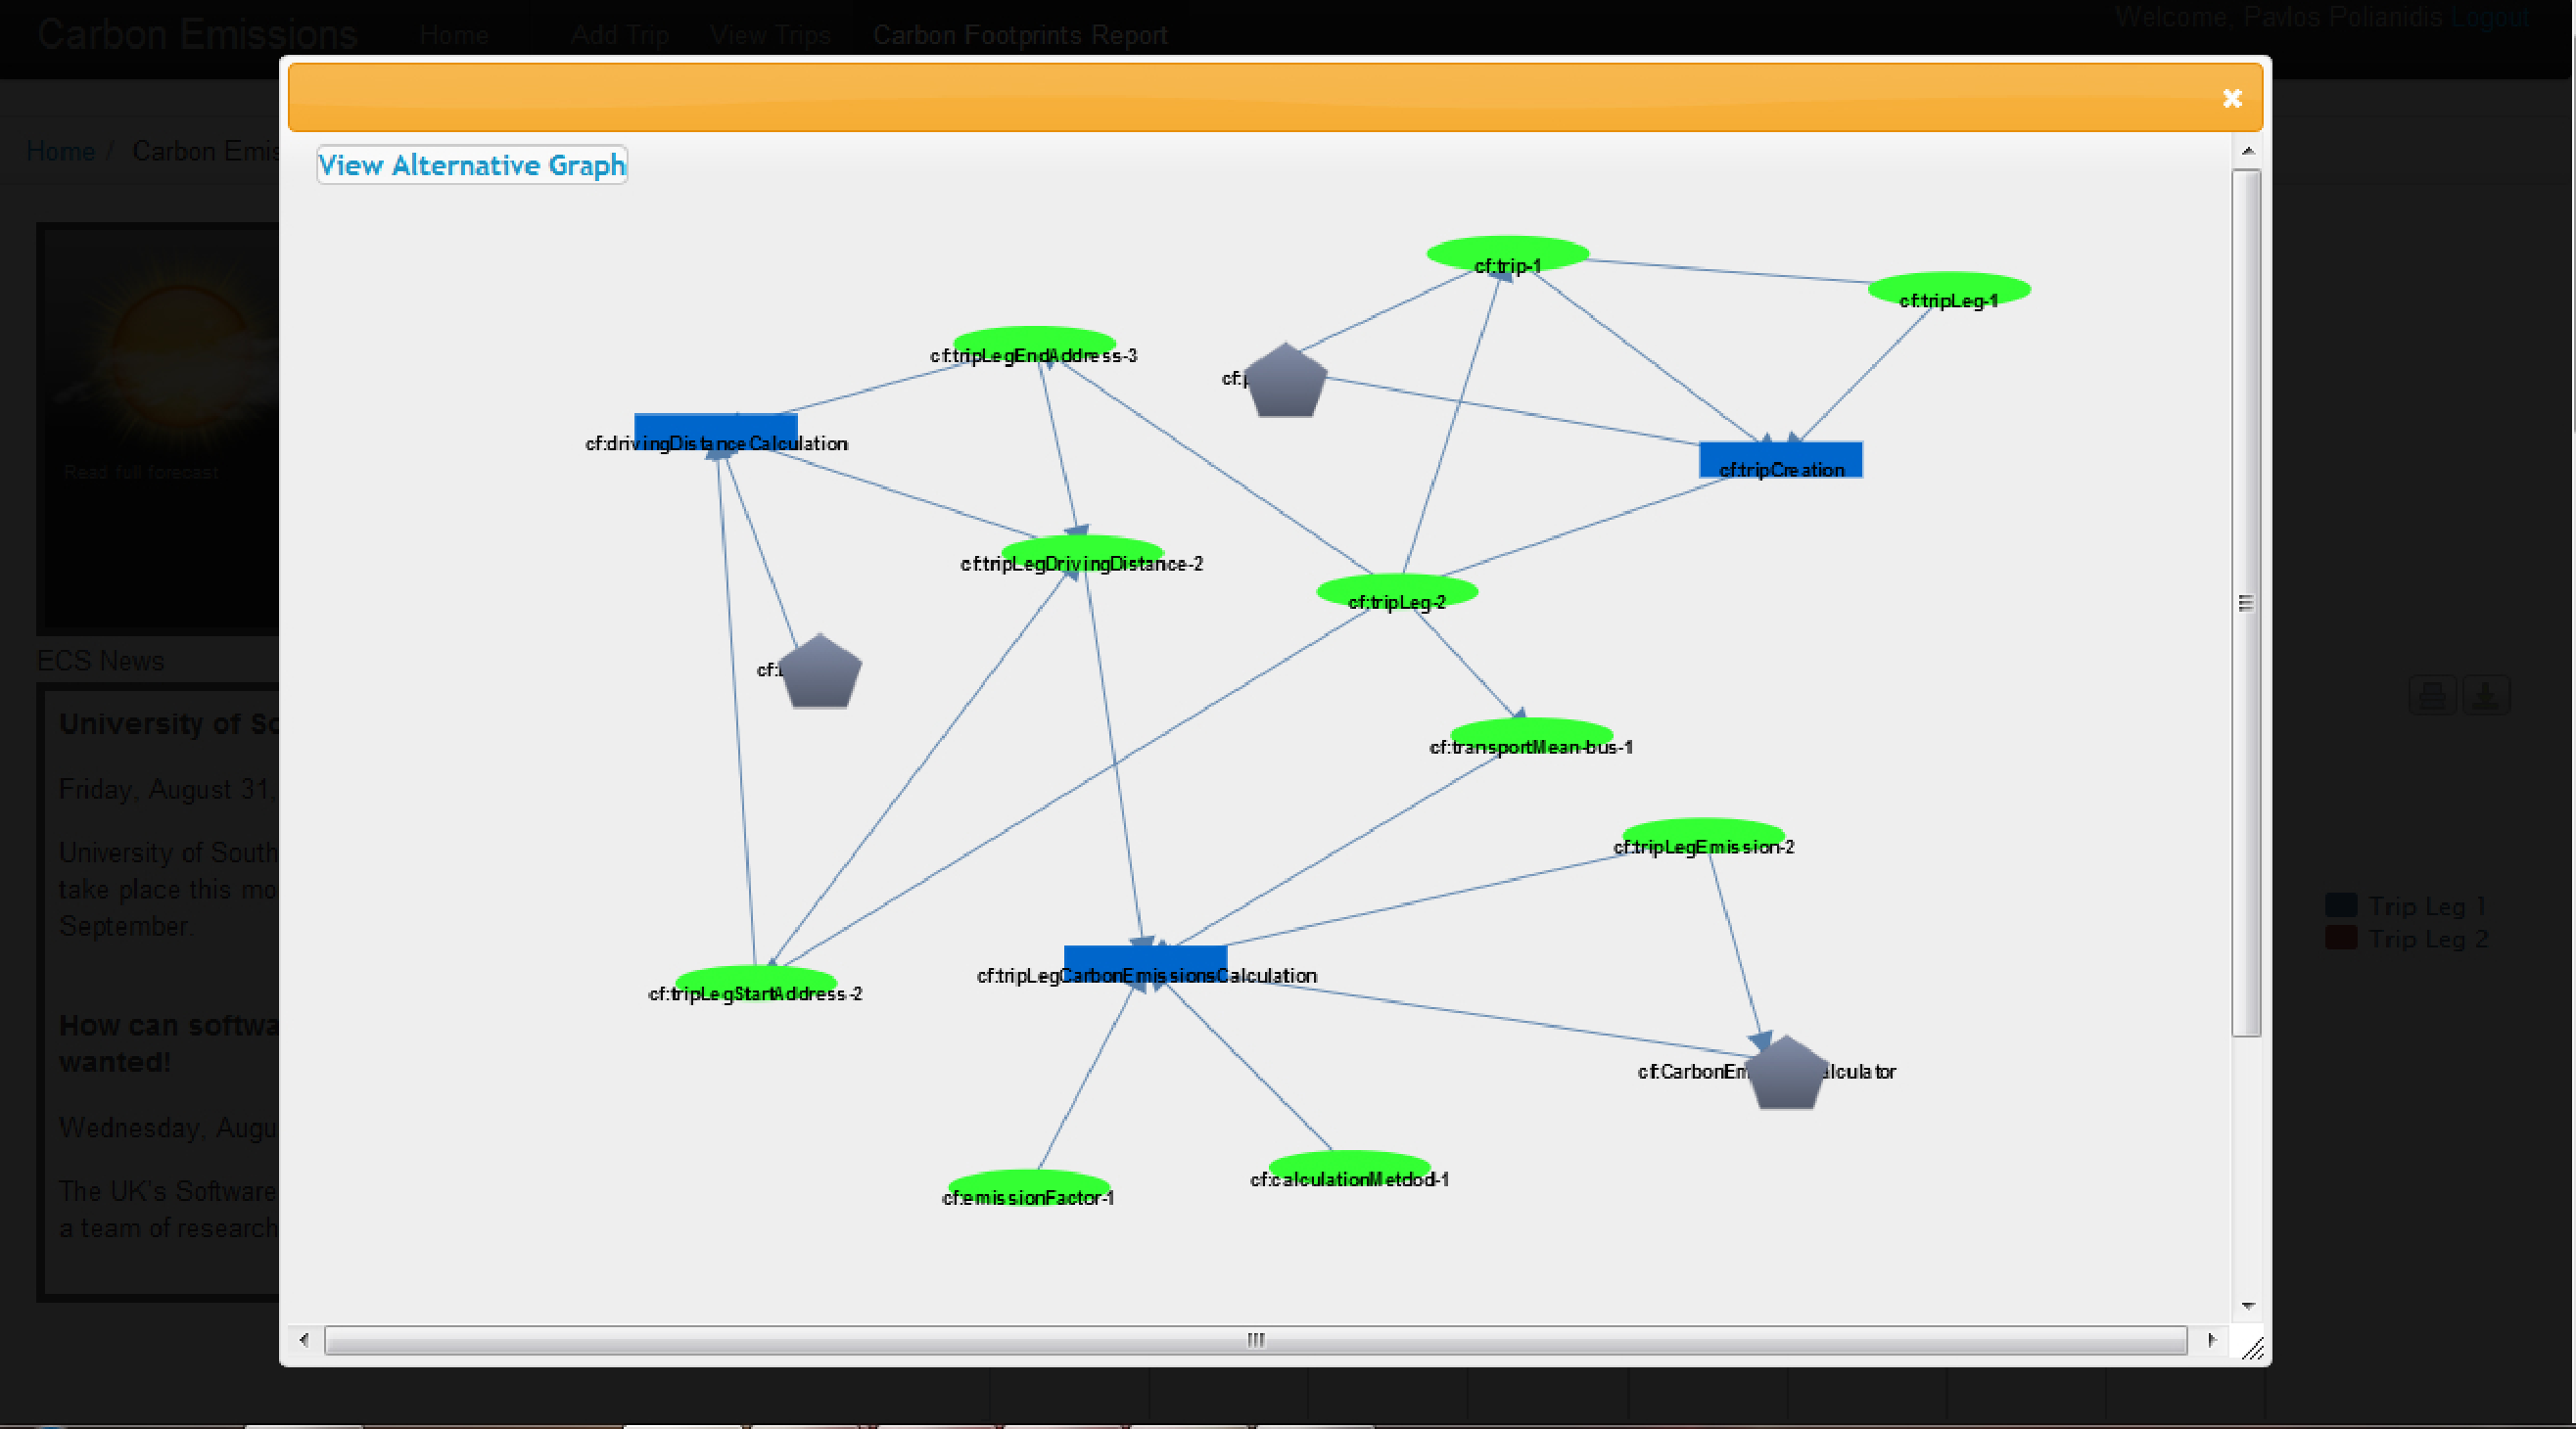
\includegraphics[scale=0.40]{./Figures/chapter4/figure18.pdf}
		\rule{35em}{0.5pt}
	\caption[Interactive provenance graph]{Interactive provenance graph}
	\label{fig:provGraph}
\end{figure}

It is obvious that the interactivity comes at the cost of a non-intuitive visualization. That is to say, the graph is not very readable, unless user relocate manually all the nodes. As a result, a second static graph is provided (figure \ref{fig:provStaticGraph}).

\begin{figure}[htbp]
	\centering
		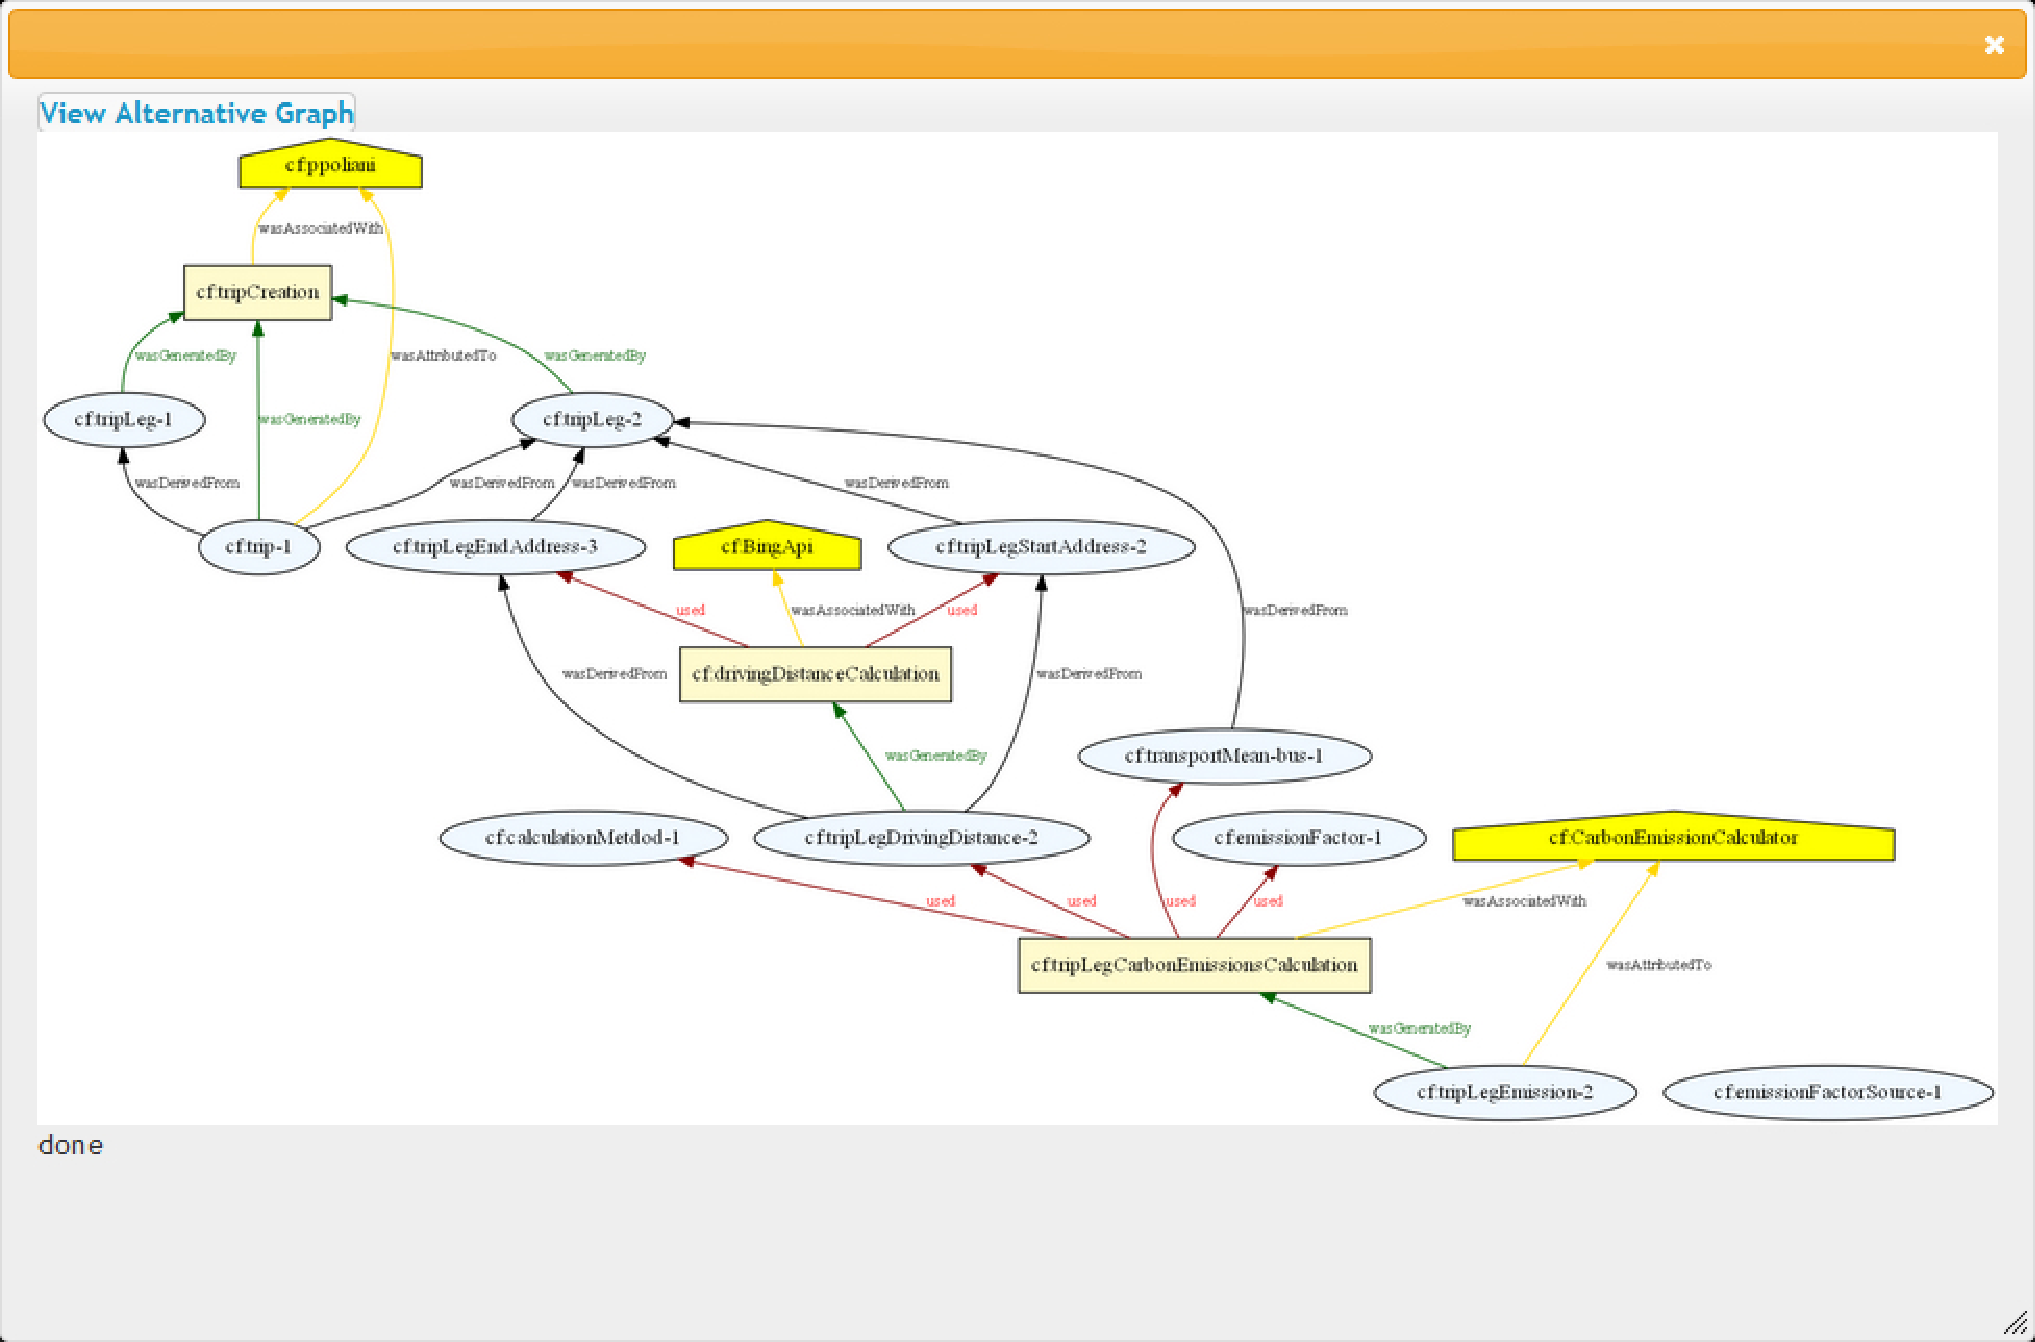
\includegraphics[scale=0.50]{./Figures/chapter4/figure19.pdf}
		\rule{35em}{0.5pt}
	\caption[Static provenance graph]{Static provenance graph}
	\label{fig:provStaticGraph}
\end{figure}

Greenhouse gas emissions can be summarized at the level of trips, as well. \emph{The GHG Emissions Per trip} line chart (figure \ref{fig:ghgPerTrip}), visualizes the weight of ghg emissions for each trip user made, during a specified period of time.

\begin{figure}[htbp]
	\centering
		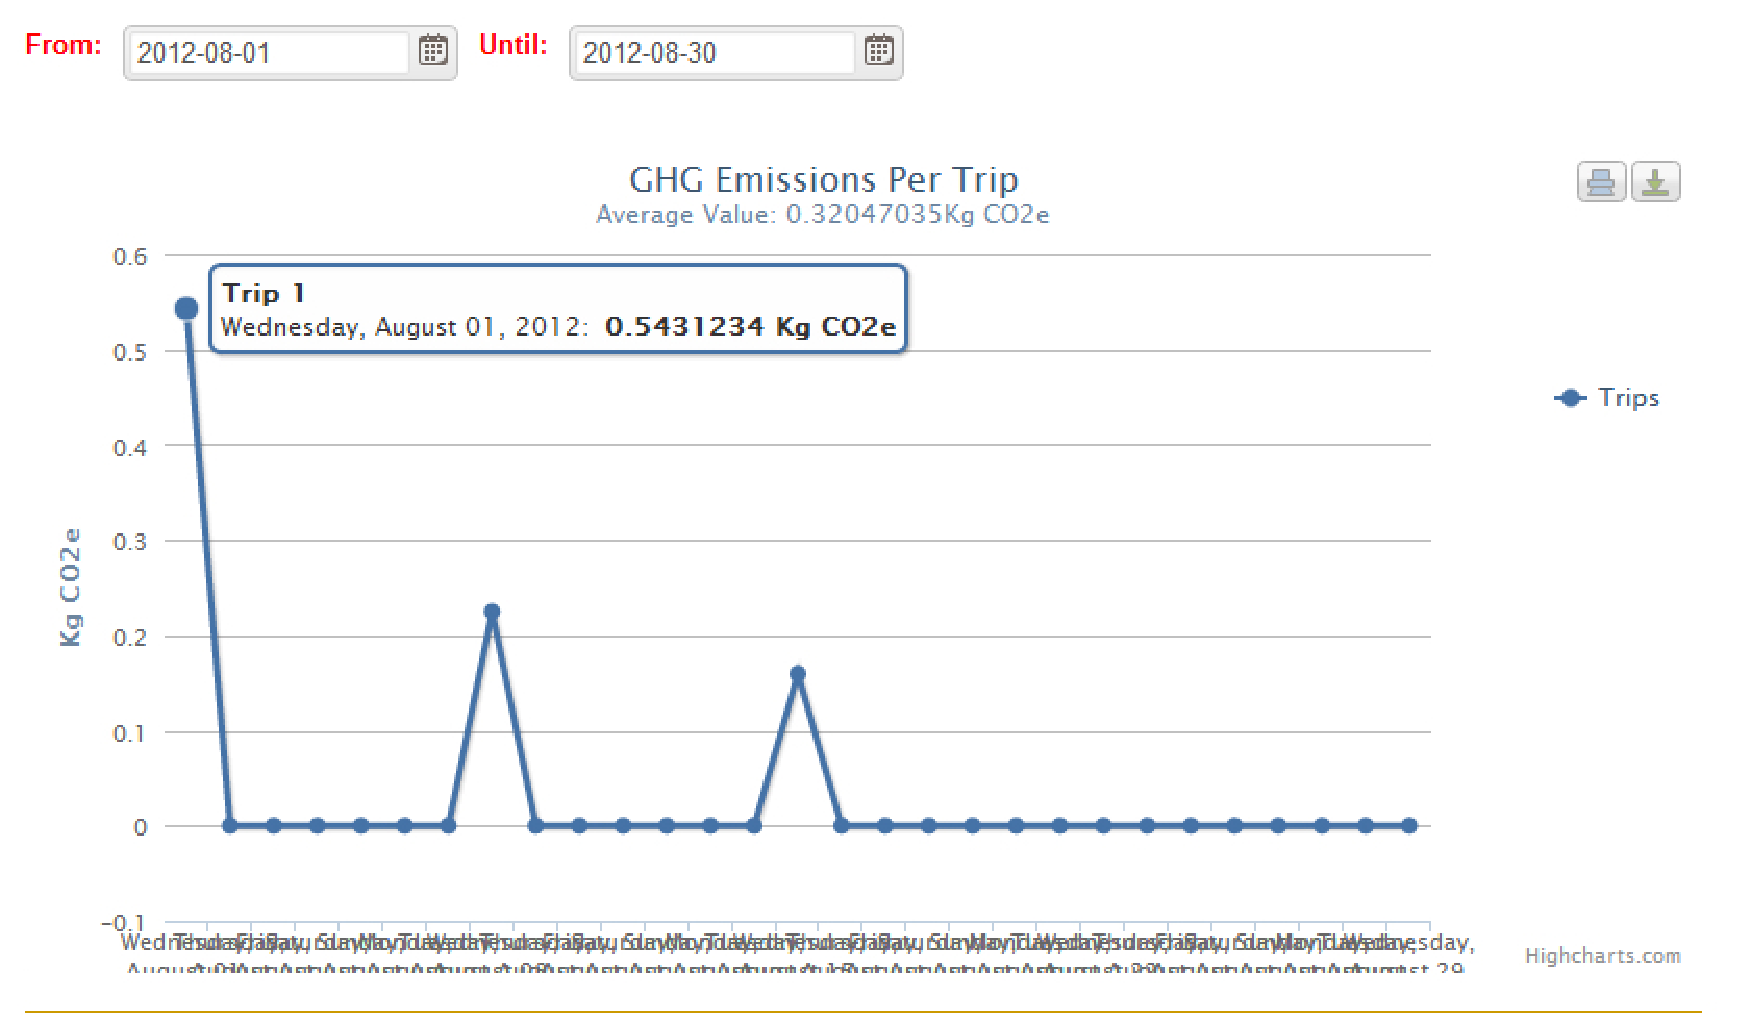
\includegraphics[scale=0.60]{./Figures/chapter4/figure20.pdf}
		\rule{35em}{0.5pt}
	\caption[Greenhouse gas emissions per trip leg]{Greenhouse gas emissions per trip leg}
	\label{fig:ghgPerTrip}
\end{figure}

The last chart (figure \ref{fig:ghgPerTransportMean}) pertaining to individual carbon footprints, illustrates the weight of carbon emissions caused by the different modes of transports, which were used during the trips made within a specified period of time.


\begin{figure}[htbp]
	\centering
		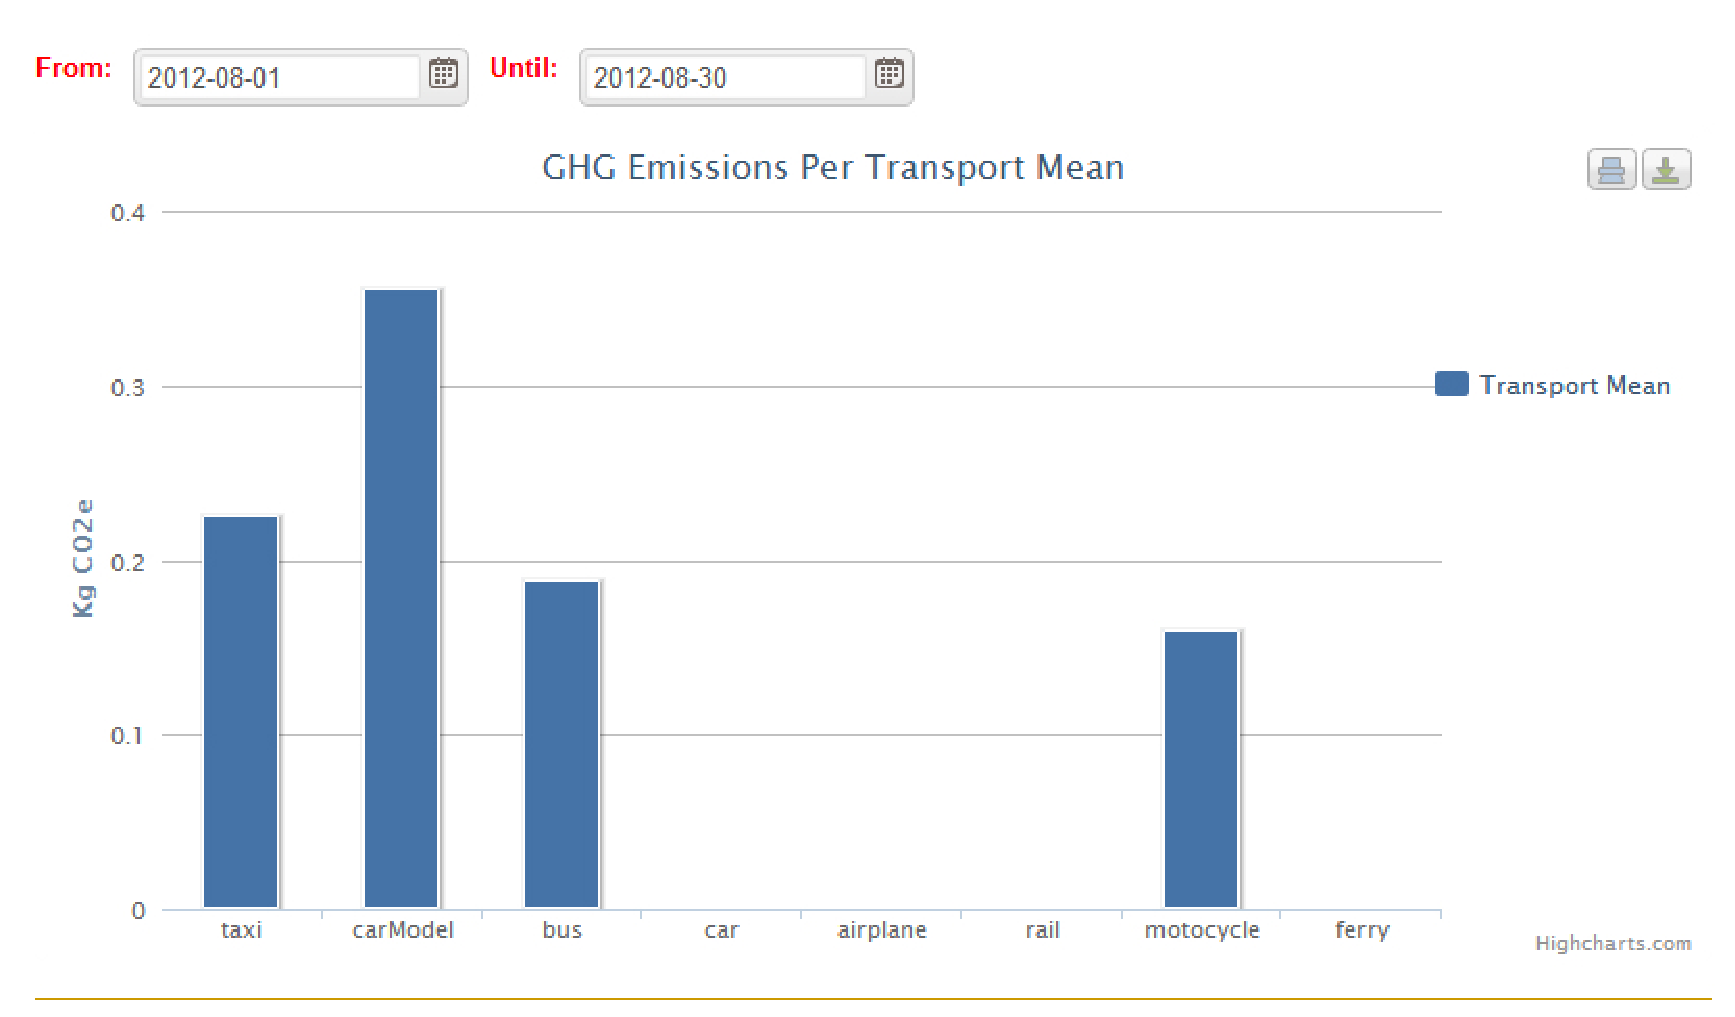
\includegraphics[scale=0.60]{./Figures/chapter4/figure21.pdf}
		\rule{35em}{0.5pt}
	\caption[Greenhouse gas emissions per transport mean]{Greenhouse gas emissions per transport mean}
	\label{fig:ghgPerTransportMean}
\end{figure}

\subsubsection{Group Carbon Emissions}

It was a initial requirement that users can be members of different groups and that carbon emissions of those groups are trackable. Consequently, aside from individual carbon footprint report, the application presents a report for users' groups. The information is similar to that enclosed in the individual report.

\begin{itemize}
  \item The number of trips that were made by the members of all user's groups.
  \item The total weight of greenhouse gas emissions (ghg) caused by all trips made by the members of all user's groups
  \item The minimum value of greenhouse gas emissions.
  \item The maximum value of greenhouse gas emissions.
  \item The average weight of greenhouse gas emissions (ghg) caused by all trips made by the members of all user's groups
\end{itemize}

\begin{figure}[htbp]
	\centering
		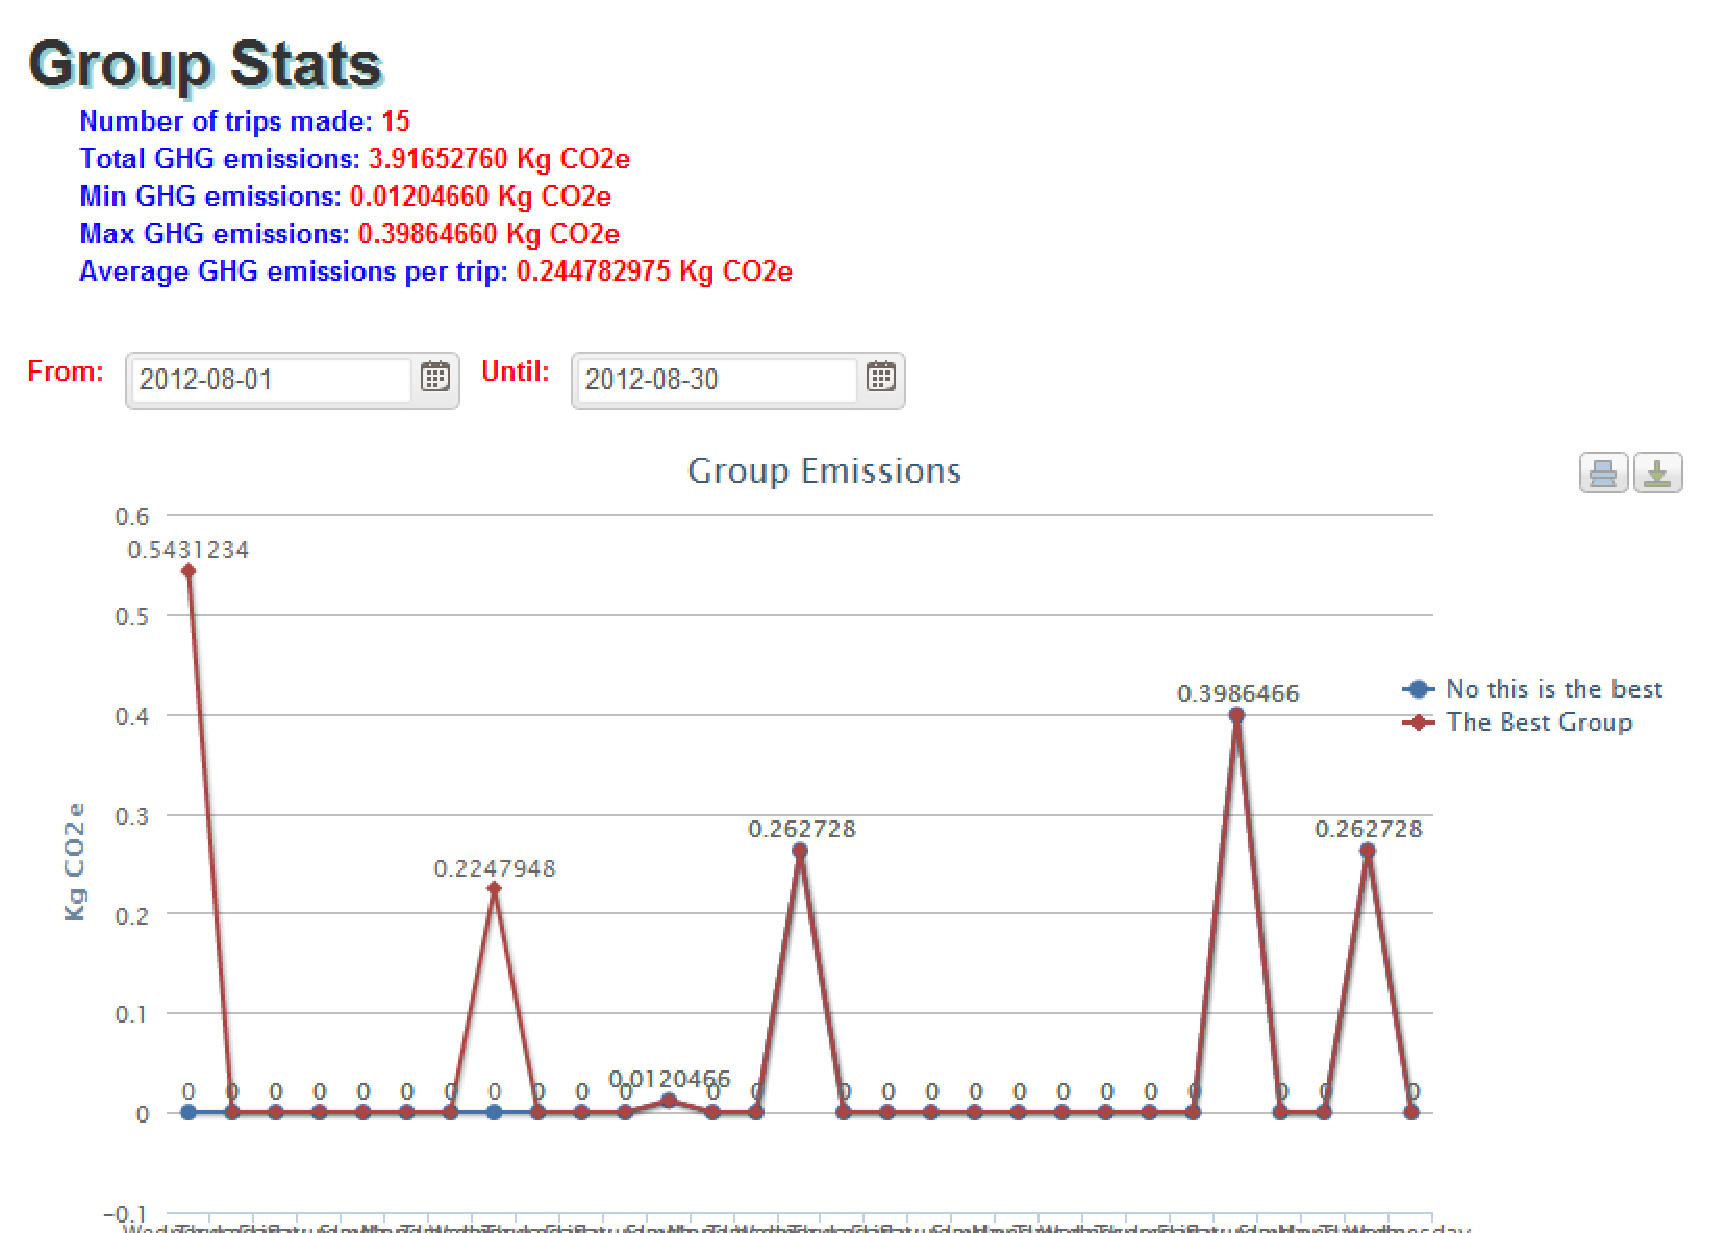
\includegraphics[scale=0.60]{./Figures/chapter4/figure22.pdf}
		\rule{35em}{0.5pt}
	\caption[Group greenhouse gas emissions]{Group greenhouse gas emissions}
	\label{fig:groupGhgEmissions}
\end{figure}


\section{Evaluation via Testing}

An initial requirement after finishing implementing the application was to get users try it and express their experience. However, this requirement changed and we tried to evaluate the system solely via tests. That is to say, each and every implemented functionality was accompanied by a unit test to verify that there are no bugs in the code. Furthermore, a series of accessibility and usability checks were performed. This section outlines the a subset of unit tests that were performed, as well as, presents the results of the accessibility and usability test.

\subsection{Unit Testing}

The prime reason for testing the application's code, is to verify that every piece of functionality is in accordance with the system's requirements. The majority of the unit tests we present here, refer to verifying the correct data insertion into the database. To that end, we utilized the Django's built-in unit test framework. The advantage of this decision is that there is no need to pollute the database with testing data, since the framework is capable of creating a temporary test database which is destroyed at the end of the testing process.

The function that is presented below consists of several actions taken before the execution of unit tests. In particular, those actions refer to setting up the tables of the database with some initial records that are ultimately being tested.

\begin{verbatim}
def setUp(self):
    self.user = User.objects.create(username='ppoliani')
    self.userProfile = models.UserProfile.objects.create(user=self.user, title='Mr', \
        type='student', occupation='student')

    self.address = models.Address.objects.create(country='UK', county='Hampshire', \
        city='Southampton', street='723 portswood road' ,postalCode='SO17 3ST', \
        longitude = 123.6765, latitude= 123.675, name='some name', visibility=False)
    self.trip = models.Trip.objects.create(userProfile=self.userProfile,
        type='commuter', name='trip name', date=datetime.now())
    self.car = models.Car.objects.create(manufacturer='Audi', model='A5',
        engineCapacity=2000, fuelType='petrol')
    self.tripLeg = models.TripLeg.objects.create(trip=self.trip,\
        startAddress=self.address, endAddress=self.address, transportMean=self.car,\
        step=1, time=datetime.time(datetime.now()))
    self.transportMeanUsedByUser =
        models.TransportMeansUsedByUsers.objects.create(transportMean=self.car,\
        userProfile=self.userProfile)

    self.emissionFactorSource =
        models.EmissionFactorSource.objects.create(name='Defra', year=2012,\
        link='http://link.com')
    self.emissionFactor =
        models.CarEmissionFactor.objects.create(source=self.emissionFactorSource,
        directGHGEmissions=0.1232, fuelType='petrol', carType='small car')

    self.transportMeanEmissionFactor =
        models.TransportMeanEmissionFactor.objects.create(transportMean=self.car, \
        emissionFactor=self.emissionFactor)
    self.calculationMethod =
        models.C02CalculationMethod.objects.create(name='tier1 method', \
        description='some description', tier='1')

\end{verbatim}

The list below summarizes a subset of the unit tests that were performed during the application's implementation phase.


\begin{verbatim}
def test_insertingUserProfiles(self):
    #passes
    self.assertEqual(self.user.get_profile().title,'Mr')

    #fails
    self.assertEqual(self.user.get_profile().type,'academic')
\end{verbatim}

The $test\_insertingUserProfiles$ unit test verifies that insertions into table \emph{UserProfiles} are performed without any errors. The first assertion must pass because in the set up function we stored a user who has the title Mr. Whereas, the second assertion fails because the type of the inserted user is student and not academic.



\begin{verbatim}
def test_insertAddresses(self):
    #passes
    self.assertEqual(self.address.country,'UK')

    #fails
    self.assertEqual(self.address.city,'London')
\end{verbatim}

The $test\_insertAddresses$ unit test verifies that insertions into table \emph{Addresses} are performed without any errors. The first assertion passes because we inserted an address with the value UK for the property country. Accordingly, the second assertion fails because the city of that address is Southampton and not London.


\begin{verbatim}
def test_insertTrips(self):
    #passes
    self.assertEqual(self.trip.name,'trip name')

    #fails
    self.assertEqual(self.trip.type, 'business')
\end{verbatim}

The $test\_insertTrips$ unit test verifies that insertions into table \emph{Trips} are performed without any errors. The first assertion is correct because the name of the trip that was inserted was indeed 'trip name'. On the other hand, the second assertion is false because a commuter type trip was inserted and not a business type.

\begin{verbatim}
def test_insertCars(self):
    #passes
    self.assertEqual(self.car.model,'A5')

    #fails
    self.assertEqual(self.car.engineCapacity, 100)
\end{verbatim}

The $test\_insertCars$ unit test verifies that insertions into table \emph{Cars} are performed without any errors. The car that was inserted has a value 'A5' for the model property and the engine capacity is 2000. As a result, the first assertion is true whereas the second is false.

\begin{verbatim}
def test_insertTripLegs(self):
    #passes
    self.assertEqual(self.tripLeg.trip.type,'commuter')
    self.assertEqual(self.tripLeg.trip.userProfile.type,'student')
    self.assertEqual(self.tripLeg.startAddress.country,'UK')

    #fails
    self.assertEqual(self.tripLeg.transportMean.engineCapacity, 3000)
\end{verbatim}

The $test\_insertTripLegs$ unit test contains multiple tests. First of all insertions into table \emph{TripLegs} are verified. In addition, connections between the TripLegs table and the \emph{Addresses}, \emph{TransportMeans} and \emph{UserProfiles} tables are checked. The first assertion is true because the the type of the trip of which this trip leg is part of, is commuter. Similarly, the second assertion is true, since the type of the user that made the trip, is student. Finally, the third assertion is true, because the country of the start address matches the value that is checked (i.e. 'UK'). On the other hand, the last assertion fails because the engine capacity of the transport mean that was used, in not 3000 but 2000.

\begin{verbatim}
def test_insertTransportMeanUsedByUsers(self):
    #passes
    self.assertEqual(self.transportMeanUsedByUser.transportMean.model,'A5')

    #fails
    self.assertEqual(self.transportMeanUsedByUser.userProfile.title, 'Miss')
\end{verbatim}

The $test\_insertTransportMeanUsedByUsers$ unit test checks that transport means used by users are correctly inserted and associated with the appropriate user. The first, assertion will pass because the model of the transport mean matches with the value checked. Similarly, the second assertion will fail because the title of the user that used that mode of transport is 'Mr' and not 'Miss'.

\begin{verbatim}
 def test_insertingTransportMeanEmissionFactors(self):
    #passes
    self.assertEqual(self.transportMeanEmissionFactor.transportMean.model, 'A5')

    #fails
    self.assertEqual(self.transportMeanEmissionFactor.emissionFactor.source.name,
        'WrongName')
\end{verbatim}

The $test\_insertingTransportMeanEmissionFactors$ unit tests checks that emissions factors are correctly connected to the corresponding transport means. Thus, the first assertion is true because we associated the emission factor with the transport mean with the value 'A5' for the model property. The second assertion checks if the conection between the \emph{EmissionsFactors}  and \emph{EmissionFactorSources} tables are properly applied. The assertion fails because the name of the emission source is 'Defra' and not 'WrongName'.

\begin{verbatim}
def test_tripLegCarbonEmissionCalculation(self):
    c = Client()

    # Extra parameters to make this a Ajax style request.
    kwargs = {
        'tripLegId':self.tripLeg.id,
        'drivingDistance': 100,
        'transportMeanType': 'car',
        'calculationMethod': 'tier1'
    }
    response = c.post('/compute-trip-leg-emissions/', kwargs)

    #pass
    emissions = float(models.TripLegCarbonEmission.objects.get(tripLeg=self.tripLeg)
        .emissions)
    self.assertEqual( emissions, 12.32)

    #fail
    self.assertEqual( emissions, 120.32)
\end{verbatim}

The $test\_tripLegCarbonEmissionCalculation$ unit test is slightly different that the previous ones. The reason is that it creates a temporary client that is capable of making HTTP POST request. In essence, it imitates an AJAX Post request to the '/compute-trip-leg-emissions/' address passing some data for computing the weight of carbon emitted during a trip leg. The first assertion is true because the expected value matches the computed one. This is exactly the reason why the second assertion fails.


\subsection{Accessibility and Usability Test}

Our application is a web based application; we therefore tried to meet several accessibility and usability requirements. Table \ref{accessUsabTest} summarizes the results of the accessibility and usability test. The test was conducted according to the guidelines published on web2access.org.uk \footnote{\url{http://www.web2access.org.uk/test}}.

\begin{table}
  \centering
  \begin{tabular}{|p{150px}|p{250px}|}
    \hline
    Test  & Result\\ \hline

    Are login, signup and other forms accessible? & Simple, accessible forms with clear labels e.g. 'username (email)' and 'password'. \\ \hline

    Are text alternatives offered for images etc? & Acceptable alternative text throughout. \\ \hline

    Is the target for every link clearly defined? & Links fully appropriate, used throughout the site plus alternative navigation element. \\ \hline

    Do frames and iframes have appropriate titles and suitable layout? & No frames or iframes used for design. \\ \hline

    Is the page fully functional and fully navigable without the stylesheet? & Content and navigation accessible. \\ \hline

    Are tables used inappropriately to format the page? & Page layout does not use tables and/or headered tables are used to present data. \\ \hline

    Is tab order logical? & Intermittent random ordering with selection jumping from one area to another. \\ \hline

    Are the pages beyond login functional and navigable with the keyboard? & Non-critical features on the page require mouse use. Maybe browser dependent i.e. works with one browser but not another. \\ \hline

    If a rich-text editor is used, is it accessible?  & Fully accessible and usable or Not Applicable. \\ \hline

    Is there appropriate feedback after submitting information and adequate time allowances? & Appropriate feedback, user directed to what they should do next, no time restrictions.\\ \hline

    Is the content comfortable to read with good colour contrast levels and no colour deficiency issues? & Site colour contrast adequate but some non-critical text in bizarre fonts or not comfortable to read \\ \hline

    Does the page maintain its style and usability when the browser zoom feature is used? & Layout and readability unaffected when zooming. \\

    Is text size and style suitably readable? Is there any blinking or flashing & Sans-serif fonts used in all body content (excludes headings). Regular font size (10/12pt) throughout and reasonable layout. \\ \hline

    \hline
  \end{tabular}
  \caption{Accessibility and usability test results}\label{accessUsabTest}
\end{table}

\section{Critical Assessment}

Having described the design and implementation of the application, we can now provide a criticism about the final outcome. The application is missing several features that were intended to be implemented, in the first place.

First of all, one of the main challenges was to design an application that would ease the task of adding new data. To that end, the initial intention was to design a user interface that would allow users to re-use the data that they have already inserted. More specifically, the process of adding new trips is relatively dull, and users would definately try to avoid it. Moreover, it is very likely that they are going to add the same trip several times; therefore, a functionality that would allow users to use the same trip again and again without the need of repeating themselves, was planed to be supported by the application. The infrastructure for implementing that feature is already there, which means that it can be easily incorporated into the current application.

Another requirement that was not met, has to do with users' input validation on client-side. Data that users insert into the \emph{trip creation form} needs to be validated, so that only the correct types of data are sent to the back-end. There was an attempt to support this feauture by utilizing a JavaScript library and the native HTML5 validation mechanism. However, the html template engine that we used (Handlebars.js) did not seem to cooperate well with those libraries. Hence, the implementation of that feature was postponed for later, but we did not consider LeBlanc's law: \emph{Later equals never}.

A  better navigation through users data was also planned to be included in the application. In the current state, the application displays users' trips categorized according to the mode of transport that was used. An additional feature would be to view trips refering to specific addresses ot trips made at a particular date.

With regards to carbon footprint report, more detailed information has to be incorporated; for instance, the corresponding trip for the minimum ghg emissions value should be indicated. However, because all the required data are already stored in the database, we consider that the implementation of such features would be easy.

Considering the provenance graphs that are presented in the carbon emission report, we need to admit that they do not cover the whole range of graphs that were planed to be implemented. Examples of graphs that are missing are: graphs that illustrate the provenance of the carbon emission values of particular trips, or graphs that display the provenance of individual's or group's carbon emissions.

It is obvious that there are several requirements that the application does not meet. The main reason for that is that a considerable amount of time was spend to design and implement the main infrastructure that would support those features. We therefore acknowledge that meeting those requirements is a matter of a few days' work, trying to bring all pieces of the puzzle together.

\section{Future Work}

There still are various features that could extend the current capabilities of the application. We need to clarify that the following list is not complete and that there might be numerous functionalities that can be added to an online carbon emission calculator.

To start with, we believe that a better solution for keeping track of users' trips would be to utilize the GPS mechanism of mobile devices.  In particular, a mobile app can record users' geo locations and make educated estimations about the mode of transports used during the trips. This way, users are not required to add any information to the system. There is a significant caveat with this approach, though.  There might emerge privacy issues, since the system would constantly know users' locations. Thus a good understanding of the possible limitations has to be acquired.

Another significant feature that might make users' life better, is to allow them make various customizations; for instance, users can pre-define a set of transport means and addresses that they usually use. Then the application could show those lists every time users add a new trip. This would make much easier and faster the process of adding trips. Furthermore, the results of carbon emission calculations could become more accurate if the users would specify the exact routes of the trips they add. Right now, the application calculates the driving distance of the default route between two addresses. In future editions, users will be able to define precisely those routes.

In terms of calculating carbon emissions, the application could use a more expanded set of calculation methods. Those methods could be added as plug-in methods to the current application. Additionally, calculation methods should be executed when missing data are provided; for instance, when users do not specify the fuel type of a transport mean.

The application can be further extended by adding a recommendation engine, which could help minimizing individual and group carbon footprints. In essence, the engine would suggest modes of transports that have low carbon emissions and are appropriate for the users' daily journeys.

Finally, an ontology for describing relationships in provenance graphs could be designed. This ontology would, essentially, be a special case of the PROV-Ontology.


\section{Summary}

In this chapter we reviewed:

\begin{itemize}
  \item 
        the implemenation of the application. For that reason, a set of sequence diagrams were given showing the execution flow of different parts of the application. Screenshots demonstrating the application's UI were also presented.
  \item
        the evaluation of the application by presenting several test cases, as well as, the results of the accessibility and usability tests. 
  \item
        some aspects of the implementation, that we could have done considered differently, and
  \item
        some additional features which believe that future versions of the application can support.
\end{itemize}
